% !TeX encoding = UTF-8
% !TeX TXS-program:compile = txs:///latexmk/{-pdf} -xelatex
% !TeX TXS-program:recompile-bibliography = txs:///latexmk/{} -v

% 载入 SJTUThesis 模版（学士学位论文：type=bachelor；jwc 为学士预设）
\documentclass[type=bachelor,preset=jwc,oneside]{sjtuthesis}
% 选项
%   type=[doctor|master|bachelor],     % 可选（默认：master），论文类型
%   zihao=[-4|5],                      % 可选（默认：-4），正文字号大小
%   lang=[zh|en|de|ja],                % 可选（默认：zh），论文的主要语言
%   review,                            % 可选（默认：关闭），盲审模式
%   [twoside|oneside],                 % 可选（默认：twoside），双页或单页边距模式
%   [openright|openany],               % 可选（默认：openright），奇数页或任意页开始新章
%   math-style=[ISO|TeX],              % 可选 (默认：ISO)，数学符号样式
%   preset=[base|jwc],                 % 可选（默认：base），预设配置，学士学位论文考虑使用 jwc 预设

% 论文基本配置，加载宏包等全局配置
% !TEX root = ./main.tex

% 模板默认 zh+en 双扉页；双面 + openright 会在英文扉页前插入空白页。
% 仅保留中文扉页时改为只含 zh（须在 \sjtusetup 之前执行）。
\ExplSyntaxOn
\clist_gset:Nn \g__sjtu_lang_clist { zh }
\ExplSyntaxOff

\sjtusetup{
  %
  %******************************
  % 注意：
  %   1. 配置里面不要出现空行
  %   2. 不需要的配置信息可以删除
  %******************************
  %
  % 信息录入
  %
  info = {%
    %
    % 标题
    %
    zh / title           = {基于 Flink 的动态 Kafka-Topic 发现与订阅机制研究},
    en / title           = {A Sample Document for \LaTeX-based SJTU Thesis Template},
    %
    % 标题页标题
    %   可使用“\\”命令手动控制换行
    %
    % zh / display-title   = {上海交通大学学位论文\\ \LaTeX{} 模板示例文档},
    % en / display-title   = {A Sample Document \\ for \LaTeX-based SJTU Thesis Template},
    %
    % 关键词
    %
    zh / keywords        = {Flink, Kafka, 动态 Topic, Sink, 流处理, 路由映射},
    en / keywords        = {SJTU, master thesis, XeTeX/LaTeX template},
    %
    % 姓名
    %
    zh / author          = {胡文杰},
    en / author          = {Mo Mo},
    %
    % 学号
    %
    id              = {522031910511},
    %
    % 指导教师
    %
    zh / supervisor      = {任锐},
    en / supervisor      = {Prof.\ Mou Mou},
    %
    % 副指导教师
    %
    % zh / assoc-supervisor  = {某某教授},
    % en / assoc-supervisor  = {Prof.\ Uom Uom},
    %
    % 联合导师
    % zh / co-supervisor     = {某某工程师},
    % en / co-supervisor     = {Engr.\ Oum Oum},
    %
    % 所属院系
    %
    zh / department      = {计算机学院},
    en / department      = {Depart of XXX},
    %
    % 专业
    %
    zh / major           = {软件工程},
    en / major           = {A Very Important Major},
    %
    % 学位
    %   除交叉学科门类外，各一级学科按所属学科门类申请学位
    %   专业学位类别按专业名称申请学位
    %   本科生不需要填写
    %
    zh / degree          = {工学学士},
    en / degree          = {Bachelor of Engineering},
    %
    % 答辩日期
    %   使用 ISO 格式 (yyyy-mm-dd)；默认为当前时间
    %
    % date                 = {2023-05-18},
    %
    % 标题页显示日期
    %   覆盖对应标题页的日期显示，原样输出
    %
    % zh / display-date    = {2023 年 5 月},
    %
    % 资助基金
    %
    % zh / fund  = {
    %                {国家 973 项目 (No.\ 2025CB000000)},
    %                {国家自然科学基金 (No.\ 81120250000)},
    %              },
    % en / fund  = {
    %                {National Basic Research Program of China (Grant No.\ 2025CB000000)},
    %                {National Natural Science Foundation of China (Grant No.\ 81120250000)},
    %              },
  },
  %
  % 风格设置
  %
  style = {%
    %
    % 关键词首行悬挂
    %
    % keywords-format = hang,
  },
  %
  % 名称设置
  %
  name = {
    % bib             = {References},
    % ack             = {谢\hspace{\ccwd}辞},
    % achv            = {攻读学位期间完成的论文},
  },
}

% 使用 BibLaTeX 处理参考文献
%   biblatex-gb7714-2015 常用选项
%     gbnamefmt=lowercase     姓名大小写由输入信息确定
%     gbpub=false             禁用出版信息缺失处理
\usepackage[backend=biber,style=gb7714-2015]{biblatex}
% 文献表字体
\renewcommand{\bibfont}{\zihao{5}\setbaselineskip{16bp}}
% 文献表条目间的间距
\setlength{\bibitemsep}{3bp plus 1pt}
% 导入参考文献数据库
\addbibresource{refs.bib}

% 脚注格式
\usepackage[perpage,bottom,hang]{footmisc}

% Provide placeholder images like `example-image-a` / `example-image-b`
\usepackage{mwe}

% 定义图片文件目录与扩展名
\graphicspath{{figures/}}
\DeclareGraphicsExtensions{.pdf,.eps,.png,.jpg,.jpeg}

% 颜色宏包
\usepackage{xcolor} 

% 确定浮动对象的位置，可以使用 [H]，强制将浮动对象放到这里（可能效果很差）
% \usepackage{float}

% 固定宽度的表格
% \usepackage{tabularx}

% 使用三线表：toprule，midrule，bottomrule。
\usepackage{booktabs}

% 表格中支持跨行
\usepackage{multirow}

% 表格中数字按小数点对齐
\usepackage{dcolumn}
\newcolumntype{d}[1]{D{.}{.}{#1}}

% 使用长表格
\usepackage{longtable}

% 附带脚注的表格
\usepackage{threeparttable}

% 附带脚注的长表格
\usepackage{threeparttablex}

% 算法环境宏包
\usepackage[ruled,vlined,linesnumbered]{algorithm2e}
% \usepackage{algorithm, algorithmicx, algpseudocode}

% 代码环境宏包
\usepackage{listings}
\lstdefinestyle{lstStyleCode}{%
  aboveskip         = \medskipamount,
  belowskip         = \medskipamount,
  basicstyle        = \ttfamily\zihao{-5}\setbaselineskip{12bp},
  commentstyle      = \slshape\color{black!60},
  stringstyle       = \color{green!40!black!100},
  keywordstyle      = \bfseries\color{blue!50!black},
  extendedchars     = false,
  upquote           = true,
  tabsize           = 2,
  showstringspaces  = false,
  xleftmargin       = 1em,
  xrightmargin      = 1em,
  breaklines        = true,
  framexleftmargin  = 1em,
  framexrightmargin = 1em,
  backgroundcolor   = \color{gray!10},
  columns           = flexible,
  keepspaces        = true,
  % texcl             = true,  % 代码中的注释部分将会被视为 LaTeX 正文模式内容
  % mathescape        = true,  % 代码中$..$的部分将会被视为 LaTeX 数学模式内容
}
\lstnewenvironment{codeblock}[1][]{%
  \lstset{style=lstStyleCode,#1}}{}

% 直立体数学符号
\providecommand{\dd}{\mathop{}\!\mathrm{d}}
\providecommand{\ee}{\mathrm{e}}
\providecommand{\ii}{\mathrm{i}}
\providecommand{\jj}{\mathrm{j}}

% 国际单位制宏包
\usepackage{siunitx}

% 定理环境宏包
\usepackage{amsthm}
% \usepackage{ntheorem}

% 绘图宏包
\usepackage{tikz}
\usetikzlibrary{arrows.meta, shapes.geometric}

% 数据图表宏包
\usepackage{pgfplots}
\pgfplotsset{compat=newest}

% 一些文档中用到的 logo
\usepackage{hologo}
\providecommand{\XeTeX}{\hologo{XeTeX}}
\providecommand{\BibLaTeX}{\textsc{Bib}\LaTeX}

% 借用 ltxdoc 里面的几个命令方便写文档
\DeclareRobustCommand\cs[1]{\texttt{\char`\\#1}}
\providecommand\pkg[1]{{\sffamily#1}}

% hyperref 宏包在最后调用
% hidelinks：不在页面上绘制链接彩色边框（目录等处否则常显示为红框）
\usepackage[hidelinks]{hyperref}

% E-mail
\providecommand{\email}[1]{\href{mailto:#1}{\urlstyle{tt}\nolinkurl{#1}}}

% Give TeX a little extra room to break long mixed Chinese/identifier lines.
\setlength{\emergencystretch}{3em}

% 双面 openright 时，模板在 \cleardoublepage 插入的空白页上使用 \thispagestyle{empty}，
% 故无页眉页码；改为与普通页一致（仍无正文，仅恢复页眉页码）
\makeatletter
\RenewDocumentCommand \cleardoublepage { }
  {%
    \clearpage
    \if@twoside
      \ifodd\c@page
      \else
        \hbox{}%
        \newpage
        \if@twocolumn
          \hbox{}%
          \newpage
        \fi
      \fi
    \fi
  }
\makeatother


\begin{document}
\setlength{\baselineskip}{20pt}

%TC:ignore

% 标题页
\maketitle

% 原创性声明及使用授权书
\copyrightpage
% 插入外置原创性声明及使用授权书
% 此时必须在导言区使用 \usepackage{pdfpages}
% \copyrightpage[file=scans/sample-copyright-a.pdf]

% 前置部分
\frontmatter
{
\fancyhead[LE,RO]{}

% 摘要
\ctexset{chapter={afterskip=26bp}}
% !TEX root = ../main.tex

\begin{abstract}[zh]
  在云原生与事件驱动架构广泛应用的背景下，Apache Flink 与 Apache Kafka 的组合已成为实时数据流水线的常见实现方式。
  然而，现有 Flink Kafka Sink 多采用静态配置模式，作业启动后目标 Topic 与相关连接信息通常被固化；
  当下游 Kafka 拓扑因扩容、迁移、容灾切换或业务演进而发生变化时，往往需要停机修改配置并重新部署，
  从而增加运维成本并削弱实时链路的连续性。相比之下，社区在消费端已经探索了动态 Kafka Source，
  而生产端动态 Sink 的研究与实现仍相对不足。

  本文围绕“基于 Flink 的动态 Kafka Topic 发现与订阅机制”展开研究。首先，从统一 Sink API、
  Kafka 元数据访问与静态 KafkaSink 的使用方式出发，分析其在动态写入场景下的局限；
  其次，结合开题报告与中期实现，提出基于正则表达式的 Topic 发现方案，以及逻辑路由与物理路由分离的设计思路；
  在此基础上，依托现有代码实现了 DynamicKafkaSink、DynamicKafkaSinkWriter、
  SingleClusterTopicMetadataService、DynamicKafkaSinkWriterState、DynamicKafkaCommittable
  与 DynamicKafkaCommitter 等关键组件，并通过广播状态与 route 更新事件支持运行期动态路由。
  该原型能够在不重启 Flink 作业的前提下发现符合规则的 Topic、建立对应写入路径，并完成多目标写入与初步状态恢复。

  目前，系统已在本地环境完成基本功能验证，验证了动态 Topic 发现、显式 route 更新与多目标写入机制的可行性。
  同时，本文也对当前实现中的局限进行了分析，包括元数据轮询开销、失效 route 的 writer 回收不足、
  Exactly-once 语义验证尚不完整等问题。后续工作将围绕元数据访问优化、资源管理、故障恢复一致性验证
  及与静态 Sink 的对比实验继续推进。
\end{abstract}


{
\ctexset{chapter={afterskip=26bp}}
\makeatletter
\@ifundefined{cftchapfont}{}{\renewcommand{\cftchapfont}{\zihao{4}\bfseries}}
\@ifundefined{cftsecfont}{}{\renewcommand{\cftsecfont}{\zihao{-4}}}
\@ifundefined{cftsubsecfont}{}{\renewcommand{\cftsubsecfont}{\zihao{5}}}
\makeatother
% 目录
\tableofcontents
}
}
% 以下前置索引暂时不输出（contents/nomenclature.tex 等文件保留，需要时取消注释）
% 插图索引
% \listoffigures
% 表格索引
% \listoftables
% 算法索引
% \listofalgorithms
% 符号对照表
% \input{contents/nomenclature}

%TC:endignore

% 主体部分
\mainmatter

% 正文内容
{
\ctexset{chapter={afterskip=26bp}}
% !TEX root = ../main.tex

\chapter{绪论}

\section{研究背景}

在云原生、微服务与事件驱动架构广泛落地的背景下，企业核心业务越来越依赖流式数据基础设施完成日志采集、
行为分析、风控告警、实时推荐与在线监控等任务。Apache Kafka 作为分布式消息系统，凭借高吞吐、
可扩展与可持久化日志模型，被广泛部署在数据接入层与消息总线层；Apache Flink 则通过统一流批处理引擎、
有状态计算与 Checkpoint 容错机制，成为实时计算层的重要代表\cite{kreps2011kafka,carbone2015flink}。
二者的组合已经成为构建实时数据流水线的事实标准之一。

然而，生产环境中的实时链路并非始终保持静态。随着业务扩张与部署形态演进，Kafka 集群经常面临扩容、
Broker 迁移、Topic 拆分合并、跨集群灰度切换与容灾演练等变化。尤其在多租户或按业务线建 Topic 的系统中，
Topic 往往不是“预先固定、长期不变”的，而是会随着业务上线、租户新增、日期滚动或分域治理而动态增长。
与此相对，上层 Flink 作业又常常承担 7×24 小时持续运行的职责，频繁停机重启不仅会增加运维负担，
还可能影响数据链路连续性，带来重复写入、空窗期或恢复复杂度上升等问题。

从现有连接器能力看，Flink 官方 Kafka Sink 的主流使用方式仍以静态配置为主：在作业构建阶段指定目标 Topic、
bootstrap servers、序列化器与投递语义，后续运行期间若底层目标发生变化，通常需要停止作业、更新配置、
重新提交\cite{flinkKafkaDocs,flinkUnifiedSink}。这种模式在拓扑稳定场景下简单可靠，但在 Topic 动态变化的场景中，
会明显暴露出灵活性不足的问题。特别是在业务希望“持续写入、自动扩展、无需停机”的情况下，
静态 Sink 难以满足运维与业务上的双重要求。

\begin{figure}[htbp]
  \centering
  \safeincludegraphics[width=0.92\textwidth]{offline_vs_regex_routing.png}
  \caption{传统离线更新方式与基于正则的动态路由方式对比}
  \label{fig:intro-offline-vs-regex}
\end{figure}

如图~\ref{fig:intro-offline-vs-regex} 所示，传统方案通常要求在目标 Sink 变化后停止作业、修改逻辑并重新部署，
其更新过程与业务写入链路强耦合；而基于模式匹配与动态路由的方案，则能够把“写到哪里”从固定配置中剥离出来，
使作业在持续运行期间感知新目标并完成写入路径调整。这一对比也直观说明了本文课题的核心目标，
即通过动态化机制降低停机更新对实时链路的破坏。

值得注意的是，动态能力并非完全没有先例。社区已经在 Source 侧推进了 FLIP-246\cite{flip246}，
探索按模式动态发现 Kafka Topic 并调整订阅集合；生产端 Sink 方向上，FLIP-515\cite{flip515} 等讨论也表明，
业界已经意识到“动态写入目标”是值得单独研究的问题。但与消费端相比，Sink 侧除了要解决元数据发现，
还必须处理 producer 配置、目标 Topic 绑定、writer 生命周期管理、状态快照与提交语义等一系列更复杂的问题。
正是这一现实差距，构成了本文选题的直接背景。

\section{研究意义}

本课题的意义主要体现在工程实践与技术方法两个层面。

从工程实践角度看，若能够在 Flink Kafka Sink 中引入运行期动态发现与动态写入能力，
则实时作业在面对 Topic 增删、规则扩展或路由调整时，就不再必须依赖人工停机修改配置。
这对于持续运行的流处理业务具有直接价值：一方面可以降低人工介入频率，缩短配置变更到生效之间的等待时间；
另一方面有助于减少由于作业重启而产生的链路抖动、运维窗口与恢复成本。在大规模数据平台中，
这种“下游拓扑可变、上游作业不停”的能力，具有明显的工程收益。

从技术方法角度看，动态 Sink 并不是对静态 Sink 的简单封装，而是涉及元数据发现、逻辑路由与物理 Topic 映射、
底层 writer 的懒创建与复用、Checkpoint 状态快照、route 级提交与恢复等多个环节的协同设计。
因此，研究这一问题不仅能补足 Flink Kafka 集成中的一类能力空白，也能为“如何在统一 Sink API 约束下扩展动态行为”
提供一条可复用的实现路径。特别是把动态发现与已有容错机制结合起来，对后续其它动态连接器或动态外部系统适配方案，
也具有一定借鉴意义。

此外，从本科毕业设计的角度，本课题既包含对 Flink、Kafka 与连接器框架的理论学习，
也包含实际代码实现、配置管理、实验验证与系统分析，具备较强的综合训练价值。

\section{国内外研究现状}

\subsection{Kafka 与消息系统相关研究}

Kafka 通过 Topic、分区、副本与消费者组等机制支撑高吞吐消息发布订阅\cite{kreps2011kafka}。
围绕 Kafka 自身的性能与运维，已有研究从配置优化、分区策略、性能建模与负载均衡等角度改进消息系统能力：
例如，DMGA-PSO 等方法尝试对分布式消息系统配置进行自动化调优\cite{ma2025dmga}，
Astraea Partitioner 关注基于历史负载信息的 Kafka 集群节点动态负载平衡\cite{wang2022astraea}，
LogP 性能模型相关工作则从通信模型角度刻画 Kafka 性能特征\cite{wu2021logp}。
这些研究的共同贡献在于提升 Kafka 作为消息基础设施的吞吐、负载均衡与可观测性，
为上层实时计算提供了稳定的数据通道。

然而，上述工作主要把 Kafka 作为独立消息系统进行优化，其核心对象是 broker、分区或客户端负载，
并不直接解决“Flink 作业运行期间目标 Topic 集合发生变化时，Sink 侧如何自动发现并调整写入路径”的问题。
Kafka 本身提供了元数据访问、生产者事务和可提交读等底层能力，但这些能力只是动态 Sink 的构建材料；
如何在流处理连接器中把元数据刷新、生产者生命周期、route 绑定、状态恢复与提交语义组织成完整机制，
仍需要在 Flink 连接器层面进一步设计。因此，Kafka 相关研究说明了本文问题的基础设施背景，
但尚未给出面向 Flink Sink 侧动态写入的直接方案。

\subsection{Flink 流处理与连接器研究}

Flink 已在统一流批处理、有状态计算和 Checkpoint 容错方面形成较完整体系\cite{carbone2015flink}。
围绕流处理系统，学术与工业界持续研究弹性伸缩、调度优化、状态迁移和能耗控制等问题：
例如，细粒度可扩展性研究关注有状态流处理系统如何更平滑地调整资源\cite{qiu2025finegrained}，
面向 Flink 的能效感知调度与两层协调负载均衡研究则从资源效率角度改进流式作业运行\cite{li2025flinkenergy}。
Twitter Storm\cite{toshniwal2014storm}、LinkedIn Samza\cite{noghabi2017samza} 等工业系统实践，
也从不同角度展示了大规模流处理管道的工程化经验。

这些工作证明，现代流处理框架已经具备长时间运行、状态管理和故障恢复能力。
但它们的主要关注点通常位于计算框架内部，即算子调度、状态迁移、资源管理和运行时容错；
对于外部系统连接器，尤其是 Sink 侧写入目标在运行期变化时的适配机制，讨论相对有限。
Flink 官方 Kafka Connector 和统一 Sink API 为外部写入提供了标准接口\cite{flinkKafkaDocs,flinkUnifiedSink}，
并支持 \id{AT_LEAST_ONCE} 与 \id{EXACTLY_ONCE} 等投递语义，但常规 Kafka Sink 仍要求在构建阶段绑定目标 Topic。
这意味着 Flink 运行时已经具备支撑动态行为的状态与提交框架，
但官方静态 Sink 使用方式尚未充分覆盖动态 Topic 发现、route 级 writer 管理和运行期目标切换。

\subsection{开源数据接入项目与动态订阅实践}

在开源生态中，Kafka Connect 提供了面向外部系统的数据集成框架，通过 source connector 和 sink connector
把数据库、文件系统、搜索引擎等系统与 Kafka 连接起来\cite{kafkaConnectDocs}；
Debezium 则基于数据库变更日志实现 CDC，并将表级变更持续写入 Kafka\cite{debeziumDocs}；
Flink CDC 项目进一步把数据库变更捕获能力接入 Flink 生态，用于构建实时数据同步和实时数仓链路\cite{flinkCdcDocs}。
这些项目的共同价值在于降低数据接入成本，使数据源或外部系统的变化能够以流的形式进入计算链路。

但从本文关注的问题看，这些项目与动态 Kafka Sink 仍存在明显差异。
Kafka Connect 和 Debezium 更强调“外部系统到 Kafka”或“Kafka 到外部系统”的通用集成，
其动态性多体现在任务配置、表捕获范围或 connector 实例管理上；Flink CDC 重点解决数据库表结构和变更日志进入 Flink 的问题。
它们并不直接面向“一个正在运行的 Flink Kafka Sink 根据 Kafka Topic 元数据变化自动扩展写入目标”
这一场景，也不需要在同一个 Flink Sink writer 内部处理多物理 Topic 的懒创建、状态封装和 route 级提交。
因此，开源项目提供了数据接入工程化的重要参照，却不能替代本文所需的 Sink 侧动态写入机制。

\subsection{动态 Topic 订阅与动态 Sink 相关工作}

在 Flink 连接器演进中，动态 Topic 已经成为明确方向。FLIP-246 提出了 Dynamic Kafka Source，
目标是在 Source 侧支持基于模式的 Kafka Topic 动态发现，并在运行期调整订阅集合\cite{flip246}。
这一工作与本文最接近之处在于都依赖 Kafka 元数据发现和正则匹配；
但 Source 侧的核心问题是分区发现、分区分配和消费进度管理，而 Sink 侧面对的是 producer 创建、
目标 Topic 绑定、写入 fan-out、底层 writer 生命周期、事务提交与恢复状态组织，两者的状态语义和失败边界并不相同。

生产端方向上，FLIP-515 已经开始讨论 Dynamic Kafka Sink 的必要性与接口形态\cite{flip515}。
这说明社区已经意识到动态写入目标并非简单配置项，而是需要在 Sink 层单独建模的问题。
不过，从公开资料看，相关讨论更多停留在设计提案与能力方向层面，
对“如何在一个可运行原型中组织正则 Topic 发现、逻辑 route 到物理 Topic 的映射、多 writer 复用、
Checkpoint 状态快照以及 \id{EXACTLY_ONCE} 事务路径”的完整实现与实验验证仍较有限。
工业实践中也有 Kafka 与 Flink 组合进行实时事件处理的案例\cite{saket2024kafkaflink}，
但其关注重点通常是流式计算逻辑和事件关联，而不是 Sink 端目标集合的运行期动态变化。

\subsection{现有工作不足与本文问题引出}

综上，现有研究和开源项目已经分别在四个层面提供了基础：Kafka 研究提升了消息系统本身的性能与可靠性；
Flink 研究提供了有状态流处理、Checkpoint 与 Sink API 等运行时基础；
Kafka Connect、Debezium 和 Flink CDC 等项目证明了数据接入工程化的重要性；
FLIP-246 与 FLIP-515 则直接表明动态 Topic 发现和动态 Sink 是社区正在关注的方向。
但是，这些工作与本文的应用背景仍存在关键差异：本文面对的是长期运行的 Flink 作业在 Sink 侧持续写入 Kafka，
且目标 Topic 会随业务或运维变化而动态出现、调整或扩展。
在该场景下，仅有 Kafka 元数据访问能力不够，仅有 Source 侧动态订阅机制不够，
仅有静态 Kafka Sink 或外部 connector 管理框架也不够。

因此，本文需要解决的核心问题可以归纳为：如何在不修改 Flink 运行时的前提下，
基于统一 Sink API 设计并实现一套 Kafka Sink 侧动态 Topic 发现与订阅机制，
使作业能够在运行期感知目标变化、维护逻辑 route 与物理 Topic 的映射、
按 route 管理底层 writer 与状态，并尽可能复用既有 KafkaSink 的写入与提交能力。
这一问题正是后续需求分析、系统设计和实验验证的出发点，
也避免了先假设“必须实现动态 Sink”再寻找理由的逻辑倒置。

\section{本文主要研究内容}

本文遵循“问题分析—方案设计—实现验证”的路径，主要工作包括：
\begin{enumerate}
  \item 分析现有基于统一 Sink API 的 Kafka Sink 在 Topic 与生产者管理上的静态性局限\cite{flinkUnifiedSink,flinkKafkaDocs}；
  \item 设计基于正则表达式的 Topic 模式、周期性元数据扫描与差异计算，形成发现—更新闭环；
  \item 提出逻辑路由与物理路由分离的映射模型，结合广播状态支持运行期路由更新；
  \item 基于现有代码实现 \id{DynamicKafkaSink}、\id{DynamicKafkaSinkWriter}、\id{SingleClusterTopicMetadataService}、
        \id{DynamicKafkaSinkWriterState}、\id{DynamicKafkaCommittable} 与 \id{DynamicKafkaCommitter} 等
        连接器核心组件，完成动态 route 管理、状态恢复与提交链路；
  \item 以 \id{app} 模块作为实验载体，对 connector 暴露出的动态发现、显式 route 更新与静态基线能力进行验证，
        并据此分析当前实现的能力边界与后续优化方向。
\end{enumerate}

\section{论文结构安排}

全文共分六章。第 1 章介绍背景、意义与相关工作；第 2 章概述 Kafka、Flink 及 Flink Kafka Connector 相关基础；
第 3 章给出需求分析与问题建模；第 4 章阐述总体架构、模块划分及动态发现、匹配、写入与路由等关键设计；
第 5 章说明实验环境、功能验证与性能对比思路；第 6 章总结全文并讨论不足与展望。

% !TEX root = ../main.tex

\chapter{相关技术与理论基础}

\section{技术综述的聚焦范围}

围绕长期运行的 Flink 作业在 Sink 侧动态组织 Kafka 写入路径这一目标，后续需求分析与系统设计主要依赖三类基础：
Kafka 写入端的 Topic 元数据、事务与可见性语义，Flink 的 Checkpoint 与统一 Sink API，
以及现有开源连接器和社区提案在动态目标管理方面的能力边界。
因此，本章从这些内容展开，为后文分析动态 Sink 需求、设计 route 级 writer 管理和提交流程提供技术依据。

\section{Kafka 写入端相关机制}

\subsection{Topic 元数据与管理面访问}

Apache Kafka 的 Topic 是生产端写入目标的基本单位\cite{kreps2011kafka}。对于本文所研究的动态 Sink 而言，
关键并不是 Kafka 的完整消息模型，而是两个与后续设计直接相关的事实：第一，Topic 名称能够被用作动态写入目标的物理标识；
第二，Topic 集合可以通过管理面接口在作业运行期间被重新查询。Kafka Connect、Debezium 等开源项目也依赖 Kafka
作为数据交换底座，但它们通常把 Topic 当作 connector 配置或外部系统映射的结果\cite{kafkaConnectDocs,debeziumDocs}；
本文则需要把 Topic 集合作为运行期可变化的元数据输入，驱动 Sink writer 的创建、复用和回收。
当前原型正是利用
\id{AdminClient.listTopics()} 获取集群中可见的 Topic 名称，再把这些名称封装为
\id{KafkaStream}，供后续正则匹配与 route 解析使用。

因此，Kafka 在本文中同时扮演两种角色：一方面，它是承接 Flink 输出结果的下游消息系统；
另一方面，它又是一个需要被动态感知的外部元数据源。第 4 章中
\id{SingleClusterTopicMetadataService} 的职责，正是把 Kafka 管理面暴露出的 Topic 列表转换为连接器内部统一使用的
\id{KafkaStream} / \id{ClusterMetadata} 结构。这一点决定了本文的“动态发现”发生在 Topic 粒度，
而不是 partition 粒度或消费者组订阅粒度。

\begin{figure}[htbp]
  \centering
  \safeincludegraphics[width=0.9\textwidth]{kafka_flink_pipeline.png}
  \caption{Kafka 与 Flink 组成的典型实时数据流水线}
  \label{fig:kafka-flink-pipeline}
\end{figure}

图~\ref{fig:kafka-flink-pipeline} 展示了 Kafka 与 Flink 在实时数据链路中的典型位置：
多类数据源先汇入 Kafka，Flink 再作为中间处理与分析引擎，将结果写入下游数据汇聚系统或业务系统。
本文所研究的动态 Sink，正位于这一链路的“Flink 写出下游”位置，其目标不是替代 Kafka 或 Flink，
而是在二者集成边界上增强写入端的动态适配能力。

\subsection{Topic、Partition 与写入目标绑定}

Topic 是逻辑上的消息类别，其下可划分为多个分区以实现并行与扩展。
消息在分区内有序，分区之间相互独立。动态 Sink 的设计重点并不是重新实现 Kafka 的分区调度，
而是决定每条记录最终交给哪个 Topic 以及哪个底层 producer/writer 实例。因此，本文把 Topic 作为动态 route 的物理落点：
自动发现路径将 \id{stream_pattern} 命中的 Topic 展开为 \id{activeRouteIds}；
显式路由路径则把业务 \id{routeId} 解析为一个或多个实际 Topic。

一旦 route 被解析为具体 Topic，底层 \id{KafkaSink} 仍会按照 Kafka producer 的常规逻辑进行序列化、
分区选择和发送确认。换言之，本文并不改变 Kafka 对 partition 的写入语义，而是在 partition 选择之前增加了一层
“逻辑 route $\rightarrow$ 物理 Topic”的动态绑定。这个分层关系解释了为什么第 4 章需要在
\id{DynamicKafkaSinkWriter.createClusterWriter(...)} 中为每个物理 route 构造独立的底层 writer：
只有先把动态 route 解析成确定 Topic，后续 Kafka producer 才能按原有机制完成真正发送。

这一边界也说明了本文与 Kafka 分区优化类工作的差异。分区负载均衡或性能建模研究关注的是一个 Topic 内部或集群节点之间的负载分布
\cite{wang2022astraea,wu2021logp}，而本文关注的是写入目标集合本身会变化时，Flink Sink 如何在 Topic 粒度上重新组织 writer。
换言之，本文并不试图替代 Kafka 的分区器，而是在 Kafka 分区器发挥作用之前，先解决“本条数据应该进入哪些 Topic”。

\subsection{生产者事务、精准一次语义与可提交读}

本文后续涉及 \id{EXACTLY_ONCE} 验证，因此需要明确 Kafka 写入端一致性语义的边界。Kafka 的普通 producer
只能保证记录成功发送到 broker，并不能天然避免故障重试导致的重复写入。为减少重试重复，Kafka 引入了幂等 producer；
而要把一组写入作为事务提交或回滚，则需要配置 \id{transactional.id}，由 producer 在事务边界内写入记录，
并最终执行 commit 或 abort\cite{kafkaSemantics}。

事务提交后，Kafka 消费端还需要通过隔离级别决定是否读取未提交数据。\id{isolation.level=read_committed}
表示消费者只读取已经提交的事务数据以及非事务数据；\id{read_uncommitted} 则可能读到尚未提交、后续也可能被回滚的记录。
这一点对本文实验具有直接意义：如果只查看 topic offset 或使用默认消费配置，可能只能说明 broker 收到了数据，
但不足以严格证明事务数据已对下游以 committed 形式可见。因此，第 5 章在说明事务路径可运行性验证时，
关注的是 Checkpoint 成功、事务提交未报错以及目标 Topic 出现 committed 输出，而不是把其等同于完整故障注入下的端到端精准一次证明。

对于动态 Sink 来说，Kafka 事务还带来额外复杂性：静态 Sink 通常只需要围绕固定 Topic 和固定事务前缀维护 producer；
动态 Sink 则可能在运行期新增或移除 route。如果多个物理 route 共用同一事务标识，提交和恢复时容易混淆不同目标的事务边界。
因此，本文实现采用 route 级事务前缀派生策略，即由全局 \id{transactionalIdPrefix} 和 \id{routeId} 生成不同物理 route 的事务前缀。
第 4 章中 \id{buildTransactionalIdPrefix(routeId)}、\id{DynamicKafkaCommittable} 与
\id{DynamicKafkaCommitter} 的设计，正是建立在这一 Kafka 事务模型之上。

从现有能力看，Kafka 已经提供事务 producer 与 \id{read_committed} 消费隔离级别，
Flink KafkaSink 也已经能够在静态目标场景下利用这些能力实现事务提交\cite{flinkKafkaDocs,kafkaSemantics}。
但这些能力默认并不回答“运行期新增 Topic 对应的 producer 何时创建、事务前缀如何命名、旧 route 的事务状态何时能够安全释放”等问题。
这正是动态 Sink 相对静态 Sink 的特殊需求。

\section{Flink 容错与 Sink 提交机制}

\subsection{Checkpoint 与动态连接器状态}

Flink 通过 Checkpoint 与分布式快照思想实现容错\cite{carbone2015flink}。
在本文场景中，Checkpoint 需要解决的不是普通算子状态如何保存这一通用问题，而是动态连接器运行期产生的 route 状态能否被恢复。
动态 Sink 会在运行期间维护 \id{activeRouteIds}、\id{clusterWritersByRouteId}、显式 route 表以及底层 Kafka writer 状态。
如果这些信息不进入快照，作业重启后就可能丢失已经创建的写入通道，或者无法继续提交故障前产生的事务。

因此，当前代码将动态状态组织为 route 级恢复单元：\id{DynamicKafkaSinkWriterState} 记录 route 标识、
目标 cluster、Topic、事务前缀、producer 配置和底层 \id{KafkaWriterState}；
\id{DynamicKafkaSink.restoreWriter(...)} 再利用这些状态重建 route 对应的底层 writer。
这说明后文的状态设计不是为了形式上“支持 Checkpoint”，而是为了让动态 route 在故障恢复后仍能与 Kafka 写入目标重新对齐。

\subsection{统一 Sink API 与两阶段提交}

Flink 统一 Sink API 将写入逻辑拆分为 Writer、状态快照、提交前准备和 Committer 等阶段\cite{flinkKafkaDocs,flinkUnifiedSink}。
在 \id{AT_LEAST_ONCE} 语义下，Writer 通常只需保证数据被刷出到外部系统；在 \id{EXACTLY_ONCE} 语义下，
Sink 还需要与 Checkpoint 配合，把某个 Checkpoint 之前的写入作为可提交单元交给 Committer。
这也是本文没有简单地在用户函数里手动创建 Kafka producer 的原因：手写 producer 很难自然接入 Flink 的状态快照和提交回调。

当前实现中，\id{DynamicKafkaSink} 直接实现
\id{TwoPhaseCommittingStatefulSink<IN, DynamicKafkaSinkWriterState, DynamicKafkaCommittable>}。
这一选择使动态 Sink 能够在 Writer 阶段解析 route 并写入数据，在 \id{snapshotState(...)} 中保存 route 级 writer 状态，
在 \id{prepareCommit()} 中把底层 \id{KafkaCommittable} 包装为带 route 信息的
\id{DynamicKafkaCommittable}，最后由 \id{DynamicKafkaCommitter} 按 route 分组提交。
第 4 章对状态和提交路径的设计，正是对这一 API 分阶段语义的具体展开。

需要强调的是，统一 Sink API 提供的是扩展连接器的框架，而不是动态 Kafka Sink 的完整实现。
官方 KafkaSink 已经很好地覆盖了“固定目标 Topic + 指定投递语义”的主流场景\cite{flinkKafkaDocs}，
但它并不会在作业运行期间根据 Topic 正则自动扩展目标集合，也不会为逻辑 route 维护多组底层 writer。
因此，本文的研究独特性不在于重新发明 Sink API，而在于把该 API 的 Writer、状态和 Committer 阶段重新组织到 route 粒度，
使动态目标管理能够纳入 Flink 原有的容错和提交框架。

\subsection{控制流、数据流与广播状态}

本文的动态 route 验证依赖应用层广播状态：\id{DynamicJob} 读取 YAML 中的 \id{route_map}，
生成 \id{DynamicSinkEvent.update(...)} 控制事件，再通过 \id{BroadcastProcessFunction} 将 route 配置写入广播状态并转发给 Sink。
这一机制本身属于 Flink DataStream 层的能力，但它与 connector 设计密切相关：广播状态负责在进入 Sink 前过滤无效
\id{routeId}，Sink 内部则负责解释 route 更新事件并维护 \id{explicitRoutesById}。

因此，本文中的控制流与数据流不是两个完全独立的系统。控制事件和普通数据事件最终都会进入
\id{DynamicKafkaSinkWriter.write(...)}，再由 Writer 根据 \id{DynamicKafkaRouteEvent} 的语义分流。
这一点为第 3 章“控制面配置必须先于数据面生效”的需求分析提供了基础，也解释了第 4 章为什么要把
\id{DynamicKafkaRouteEvent} 设计为 Sink 可识别的统一事件接口。

\section{Flink Kafka Connector}

\subsection{静态 Kafka Sink 的目标绑定}

常规配置在作业构建阶段指定固定的 Topic 名称或静态列表，运行期不随集群侧 Topic 集合变化而自动扩展。
该方式实现简单、语义清晰，适用于拓扑稳定的场景，但在 Topic 频繁增删或按规则批量创建时，
难以避免停启作业与重复发布。本文原型中的对照组也可以理解为这种典型静态模式：
应用在作业提交前就把目标 Topic 写死到 \id{KafkaSink} 中，之后任何目标变更都需要重新构建并部署作业。
因此，静态模式更适合作为本文后续实验中的基准方案，而不是待研究问题的最终答案。

从能力边界看，静态 KafkaSink 的优势是成熟、稳定、语义清楚，尤其适合“目标已知且长期稳定”的作业。
但本文的实际需求恰好相反：目标 Topic 可能随业务上线、租户扩展或路由规则变化而出现，
且用户希望 Flink 作业不因目标变化而停机。静态 KafkaSink 无法在不重启作业的前提下重新扫描 Topic 集合，
也没有内建逻辑 route 到物理 Topic 的映射表。因此，本文把它作为复用对象和对照基线，而不是直接采用其原始形态。

\subsection{正则发现从 Source 侧到 Sink 侧的差异}

在 Source 侧，社区已支持基于正则表达式匹配 Topic 名称的订阅方式，并与分区发现、
偏移提交等机制结合\cite{flip246}。其本质是周期或事件驱动地比对“模式—当前元数据”，
更新实际订阅集合。Sink 侧若要对齐类似能力，需要另行设计生产者实例生命周期与记录路由策略，
不能简单照搬 Source 实现。本文当前代码中对“按模式发现 Topic”的实现落在
\id{DynamicKafkaSinkBuilder.setStreamPattern(...)}、\id{StreamPatternSubscriber} 与
\id{SingleClusterTopicMetadataService} 的组合上；但当模式命中新的 Topic 后，
系统还要进一步将其转换为 route id、Kafka producer 配置和底层 writer，
这一步正是 Sink 侧相较 Source 侧的主要额外复杂度。

为了更直观地对应本仓库中的实现逻辑，代码清单~\ref{code:metadata-and-pattern}
展示了当前原型中最关键的两步：先通过 \id{AdminClient.listTopics()} 拉取所有 Topic，
再通过正则对 \id{streamId} 执行匹配。这说明本文方案中的“动态发现”并不是来自
Flink 运行时的内建事件通知，而是构建在 Kafka 管理面元数据轮询之上的。

\begin{codeblock}[language=Java,caption={当前原型中的 Topic 元数据获取与正则匹配逻辑},label={code:metadata-and-pattern}]
// connector/.../SingleClusterTopicMetadataService.java
public Set<KafkaStream> getAllStreams() {
    return getAdminClient().listTopics().names().get().stream()
            .map(this::createKafkaStream)
            .collect(Collectors.toSet());
}

// connector/.../StreamPatternSubscriber.java
public Set<KafkaStream> getSubscribedStreams(KafkaMetadataService kafkaMetadataService) {
    Set<KafkaStream> allStreams = kafkaMetadataService.getAllStreams();
    List<KafkaStream> matches = new ArrayList<>();
    for (KafkaStream kafkaStream : allStreams) {
        String streamId = kafkaStream.getStreamId();
        if (streamPattern.matcher(streamId).find()) {
            matches.add(kafkaStream);
        }
    }
    return Set.copyOf(matches);
}
\end{codeblock}

结合代码可以看到，当前实现默认把 \id{streamId} 等价为 Topic 名称，因此
\id{stream_pattern} 实际上就是“对 Topic 名称做匹配”的正则表达式。这样做实现简单，
也便于原型阶段验证功能；但如果未来扩展到“逻辑流名称”与“物理 Topic 名称”并不完全一致的场景，
则需要在 \id{KafkaStream} 的建模上进一步引入更丰富的元数据层次。

\subsection{开源数据接入项目的能力边界}

除 Flink Kafka Connector 外，Kafka 生态中还存在 Kafka Connect、Debezium、Flink CDC 等成熟项目。
Kafka Connect 提供 source connector 与 sink connector 框架，用于在 Kafka 与外部系统之间搬运数据\cite{kafkaConnectDocs}；
Debezium 通过读取数据库变更日志，将表级变更持续写入 Kafka\cite{debeziumDocs}；
Flink CDC 则把变更数据捕获能力接入 Flink 作业，用于实时同步和实时数仓构建\cite{flinkCdcDocs}。
这些项目说明，开源生态已经能够很好地解决“如何把外部系统的数据接入流式链路”这一类问题。

但它们与本文需求存在本质区别。Kafka Connect 和 Debezium 的动态性主要体现在 connector 任务配置、
外部表捕获范围或任务实例管理上；Flink CDC 关注的是数据库变更如何成为 Flink 输入流。
本文则研究 Flink 作业已经在运行、数据已经进入计算链路之后，Sink 侧如何根据 Kafka Topic 元数据变化动态改变写出目标。
这一问题要求 writer 生命周期、route 状态、Kafka 事务与 Flink Checkpoint 同时协同，
并不是简单增加一个外部 connector 配置项即可解决。

\begin{table}[htbp]
  \centering
  \caption{现有方案能力边界与本文需求对比}
  \label{tab:related-capability-gap}
  \small
  \begin{tabular}{p{0.17\textwidth}p{0.29\textwidth}p{0.36\textwidth}}
    \toprule
    方案或工作 & 已具备能力 & 与本文需求的差异 \\
    \midrule
    KafkaSink & 固定 Topic 写入、投递语义、事务提交 & 目标 Topic 通常在构建阶段绑定，缺少运行期正则发现和 route 映射 \\
    FLIP-246 & Source 侧动态发现 Topic 与分区订阅 & 面向消费端 offset 和分区管理，不能直接解决 producer、writer 和提交问题 \\
    FLIP-515 & 提出动态 Sink 方向与接口讨论 & 公开资料以设计讨论为主，仍需要可运行原型和实验验证支撑 \\
    Kafka Connect 等 & 外部系统接入、CDC 与数据同步 & 关注数据进入 Kafka 或 Flink，不负责 Flink Sink 内部的动态多目标写出 \\
    \bottomrule
  \end{tabular}
\end{table}

\subsection{动态 Sink 需要解决的连接器问题}

现有 Kafka Sink 在统一 API 下仍以静态目标为主；FLIP-515\cite{flip515} 等工作讨论动态 Sink 的方向，
但生产可用的完整方案需处理：元数据扫描开销、写入路径与事务语义、状态快照与恢复后的对账等问题。
从当前原型实现看，这些难点都已经在代码层面有所体现：例如 route 级 writer 的惰性创建已经实现，
非事务路径下的退役 writer 清理也已经落地；但 \id{EXACTLY_ONCE} 路径下的安全回收、
事务边界与复杂故障验证仍待补足。
因此，Flink Kafka Connector 的“动态化”并不是单点功能，而是一组围绕 Writer、状态、提交与元数据服务的协同扩展。

结合表~\ref{tab:related-capability-gap} 可以看到，现有方案已经分别解决了静态 Kafka 写入、Source 侧动态订阅、
外部系统接入和动态 Sink 方向讨论等问题，但没有同时覆盖本文所需的四个约束：
第一，运行期根据 Kafka Topic 元数据发现目标；第二，支持业务逻辑 route 与物理 Topic 解耦；
第三，以 route 为粒度维护底层 writer、状态和提交对象；第四，在原型阶段通过实验验证发现实时性、吞吐、Checkpoint 与事务路径。
本文的独特性正来自这四个约束的组合，而不是来自某一个单独技术点。

\section{本章小结}

本章围绕后续设计所需的关键技术进行了有针对性的综述。Kafka 部分重点讨论 Topic 元数据、
写入目标绑定、事务型 producer、Exactly-once 与 \id{read_committed} 可见性；
Flink 部分重点说明 Checkpoint、统一 Sink API、两阶段提交和广播状态如何支撑动态连接器；
Connector 部分则对比了静态 KafkaSink、FLIP-246、FLIP-515、Kafka Connect、Debezium 与 Flink CDC 等已有工作。
可以看到，现有方案已经提供了若干可复用能力，但无法完整满足本文“Sink 侧运行期动态发现、多 route 写出、状态快照和提交协同”的组合需求。
因此，本文后续提出的动态 Kafka Sink 原型并非对通用技术的重复介绍，
而是在现有能力边界之上面向特定场景进行的连接器扩展。

% !TEX root = ../main.tex

\chapter{系统需求分析}

\section{系统应用场景分析}

在实时数据平台中，Flink 作业通常承担持续运行的计算与写出职责，而 Kafka Topic 则经常随着业务边界变化而调整。
例如，多租户系统可能按租户自动创建 Topic，日志平台可能按日期、地域或业务线拆分 Topic，
灰度迁移和容灾切换场景中也可能同时存在新旧 Topic 或新旧集群。若仍采用传统静态 Sink，
作业在提交时就把目标 Topic 与连接参数固定下来，一旦下游目标变化，就需要停止作业、修改配置并重新部署。
这一过程会引入运维窗口、恢复等待时间和潜在重复写入风险，与实时链路“持续写入、低人工介入、快速接纳新目标”的要求相矛盾。

因此，本文面对的核心问题不是“如何把数据写入一个 Kafka Topic”，而是“当可写 Topic 集合在运行期间变化时，
Flink Sink 如何在不重启作业的前提下发现变化、更新写入目标，并保持状态与提交路径可恢复”。
这一问题天然包含两个层次：第一，系统需要从 Kafka 集群元数据中识别符合规则的新 Topic；
第二，系统需要把业务侧的逻辑路由与实际物理 Topic 解耦，使业务记录不必直接绑定某个固定目标。
前者对应自动发现路径，后者对应显式逻辑路由路径。

在本项目中，connector 通过 Topic 匹配模式、路由映射和元数据发现间隔等参数暴露动态能力，
而应用层只负责把这些参数装配进运行中的 Flink 作业。
因此，系统不仅要支持“自动发现符合模式的 Topic”，还要支持“根据业务路由标识动态决定消息应写往哪一类 Topic”。
这意味着问题已从“静态写一个 Topic”扩展为“运行期维护逻辑路由、物理 Topic 与底层写入通道的关系”。

与抽象需求相对应，当前仓库中的配置已经给出了较为完整的输入形式，本文将其整理至附录~\ref{appendix:configs}。
从这些配置可以看出，该 connector 同时暴露了自动发现所需的 \id{stream_pattern} 与
\id{discovery_interval_ms}，以及显式路由所需的 \id{route_map}。这意味着本文讨论的并不是
单一路径下的动态写入，而是“自动发现路径”和“逻辑路由路径”并存的复合场景。

\section{功能需求分析}

由上述场景可知，静态 Sink 的不足并不只是一项配置不够灵活，而是会沿着“目标发现、目标选择、写入通道、状态恢复”
形成连续影响：如果系统无法发现新 Topic，就不能减少停机变更；如果无法把逻辑路由映射到物理 Topic，
业务记录仍会被固定目标约束；如果发现目标后不能自动维护写入通道，数据仍无法真正写出；如果路由状态不能进入
Checkpoint，故障恢复后又会丢失运行期动态信息。因此，本节将功能需求拆分为动态 Topic 发现、自动订阅、
动态路由和数据处理四类，它们分别对应前述问题链条中的不同环节，并共同支撑后续第 4 章的系统设计。

\subsection{动态 Topic 发现需求}

系统应能根据用户配置的 Topic 名称模式，周期性查询 Kafka 当前 Topic 列表，并识别所有符合规则的目标。
当前实现中，构建阶段接收用户配置的 Topic 匹配模式，运行期由订阅规则调用元数据服务完成匹配；
在单集群原型中，内部流标识直接等价于 Topic 名称，因此模式匹配实质上就是对集群 Topic 名称做运行期过滤。

\subsection{自动订阅需求}

Sink 侧的“订阅”不是消费者组意义上的分区订阅，而是指写入执行模块对“当前可写目标集合”的维护。
在实现中，这一集合由内部活动路由集合表示；当元数据刷新触发时，系统重新计算新的可写路由集合，再按路由标识检查是否需要创建新的底层写入通道。
因此，本系统必须支持以下功能：一是首次启动时根据元数据建立可写集合；二是在运行期发现新增路由时自动扩展写入路径；
三是在路由不再被活动集合或显式逻辑路由引用时，尽可能释放对应写入通道，避免长时间累积陈旧资源。

需要指出的是，当前代码已经支持路由的新增与切换，并在无事务和至少一次路径下补充了退役写入通道清理；
但在精准一次路径下，由于事务上下文可能跨 Checkpoint 存在，当前实现仍采用保守策略，不自动清理退役写入通道。
因此，自动订阅需求在本文原型中已经形成基本闭环，但事务路径下的安全回收仍属于后续工程化完善方向。

\subsection{动态路由需求}

系统应支持“逻辑路由标识 $\to$ 物理 Kafka 目标”的两级映射，而不是把业务记录直接绑定到固定 Topic。
在应用层，输入事件同时覆盖数据记录与路由更新两种语义：普通数据事件携带路由标识与消息内容，更新事件携带路由到目标描述的映射。
在运行时，写入执行模块会先判断输入事件属于控制面还是数据面；若是更新事件则更新逻辑路由映射；若是普通事件且显式指定了路由标识，则走逻辑路由路径。

这说明本系统的路由需求具有两个层面：其一，面向“自动发现”的通用路由；其二，面向“显式路由标识”
的逻辑路由。后者正是本文“逻辑路由与物理路由分离”设计思想的直接代码体现。

进一步地，当前原型并没有把路由配置静态地塞进 Sink，而是通过一个轻量级验证载体利用广播状态与控制事件把路由更新传播到运行中的算子实例。
图~\ref{fig:route-broadcast-flow} 展示了这一机制的关键处理逻辑：普通数据事件只有在广播状态中存在对应路由标识时才会被放行，而路由更新事件则会先改写广播状态，再继续向下游 Sink 传播。
需要强调的是，这一部分并非 connector 的核心交付物，而是为了验证 connector 的显式路由更新接口而构造的上层驱动。

\begin{figure}[htbp]
  \centering
  \begin{tikzpicture}[
    node distance=0.85cm and 1.2cm,
    box/.style={draw, rounded corners=2pt, align=center, minimum width=2.7cm, minimum height=0.8cm},
    arrow/.style={-Latex, thick}
  ]
    \node[box] (update) {路由更新事件};
    \node[box, right=of update] (write) {写入广播状态\\更新路由配置};
    \node[box, right=of write] (forward) {继续转发\\给 Sink};
    \node[box, below=of update] (data) {普通数据事件\\携带路由标识};
    \node[box, right=of data] (check) {检查广播状态\\是否存在路由};
    \node[box, right=of check] (pass) {存在则\\放行数据进入 Sink};
    \node[box, below=of check] (drop) {不存在则过滤};
    \draw[arrow] (update) -- (write);
    \draw[arrow] (write) -- (forward);
    \draw[arrow] (data) -- (check);
    \draw[arrow] (check) -- node[above, font=\small] {存在} (pass);
    \draw[arrow] (check) -- (drop);
  \end{tikzpicture}
  \caption{广播状态维护路由配置与转发流程}
  \label{fig:route-broadcast-flow}
\end{figure}

这一实现意味着系统的功能需求实际上还隐含了一个重要约束：控制面配置必须先于数据面生效，
否则普通数据即使携带了合法的逻辑路由标识，也会因为广播状态中尚不存在该路由而被过滤掉。
因此，本文在分析动态路由需求时，需要同时考虑“路由如何表示”和“路由如何传播”两个问题。

\subsection{数据处理需求}

系统应能在持续数据流上稳定完成以下处理链路：数据生成/采集、路由校验、路由解析、Topic 选择、
消息序列化、Kafka 写入、Checkpoint 快照与故障恢复。当前验证载体使用数据生成源产生测试数据，并通过广播处理逻辑先过滤掉不存在的路由标识，再将合规事件送入动态 Sink。
说明系统在验证层面已经具备“数据面”和“控制面”混合流的基本处理能力，而 connector 本身则只关心进入写入模块之后的解析、写入与状态管理。

从实现要求看，序列化层还必须适应动态 Topic 绑定。当前实现会为每个路由维护对应的序列化与目标 Topic 绑定关系，
使普通消息在保留原有 key、value 与 headers 的同时，被写入解析后的目标 Topic。
这一机制是当前原型可运行的关键约束之一。

\section{非功能需求分析}

为了避免非功能需求停留在定性描述，本文将其限定为当前原型能够在本地实验中验证的指标。
这些指标不是生产级服务等级协议，而是用于判断本文方案是否满足毕业设计原型目标的可测约束。
各项指标的取值依据来自三类因素：其一是第 3.1 节场景分析给出的业务约束，即实时链路希望在不重启作业的情况下
快速接纳新增 Topic，且动态能力不能显著破坏持续写入能力；其二是当前实现的机制上界，例如
\id{discovery_interval_ms=2000} 决定了新增 Topic 通常需要等待下一轮刷新后才能被发现；
其三是本地单机原型的实验边界，例如第 5 章采用 \id{parallelism=1}、小规模路由数量和约 30 秒运行窗口进行验证。
因此，本节中的数值不是孤立给出的，而是由“场景诉求—实现机制—实验条件”共同推导得到。

\subsection{非功能指标的推导}

首先，发现实时性指标来源于“业务目标变化后不应再以停机重启为主要生效方式”的场景诉求。
在传统静态 Sink 中，新增 Topic 往往需要修改配置并重新提交作业，生效时间通常以人工操作和作业恢复时间计。
本文原型的目标不是把发现延迟压到毫秒级，而是证明在默认轮询机制下，Topic 变化可以在一个很短的自动化窗口内被接纳。
由于实验配置采用 \id{discovery_interval_ms=2000}，理论上新增 Topic 最坏会等待接近一个刷新周期；
再考虑 Kafka 管理面查询、写入通道创建和本地任务调度开销，本文额外预留约 \id{1 s}，
因此将“首次写入不超过 \id{3 s}”作为发现实时性目标。该阈值既来自当前实现的刷新周期，又明显小于停机重启的运维窗口，
能够体现动态发现机制的实际价值。

其次，吞吐可接受性和小规模扩展性指标来源于“动态能力不应以明显牺牲稳定写入能力为代价”的场景诉求。
本文方案相比静态 KafkaSink 增加了路由查找、正则匹配结果缓存、多写入通道管理和提交对象包装，
因此完全没有开销并不现实；但在本地单机、两路由到四路由的原型规模下，这些逻辑应当只是附加管理成本，不应成为主要吞吐瓶颈。
基于这一判断，本文将动态两路由相对静态基线的吞吐下降阈值设为 5\%，用来判断动态管理层是否仍处于可接受开销范围；
将两路由增至四路由的下降阈值设为 10\%，用来观察小规模路由扩展是否立即导致写入路径退化。
若超过这些阈值，则说明路由管理、写入通道创建或提交包装已经对原型目标产生明显影响，需要在设计层面重新考虑缓存、批量刷新和写入通道复用策略。

再次，Checkpoint 协同指标来源于“动态路由状态必须进入 Flink 原生容错链路”的场景诉求。
本文并不要求本地原型达到生产集群的大规模容错性能，但要求路由级状态快照不能明显阻塞小规模作业。
在实验中 Checkpoint 间隔设置为 \id{5000 ms}，因此稳态单次 Checkpoint 若达到数百毫秒甚至秒级，
就会说明动态状态封装已经对正常流处理产生可见干扰。本文将稳态完成时延阈值设为 \id{100 ms}，
是为了保证快照耗时相对 5 秒间隔保持在较低比例内，并便于通过第 5 章日志直接观察。

最后，事务路径可运行性指标来源于“动态 Sink 不能只在至少一次语义下成立”的场景诉求。
完整精准一次语义需要故障注入、恢复验证和下游 \id{read_committed} 消费检查共同支撑，
这超出了本文本地原型实验的覆盖范围。因此本文没有把该指标定义为生产级端到端精准一次证明，
而是定义为更保守的可运行性目标：精准一次小规模运行中至少完成 5 次 Checkpoint，
并在两个目标 Topic 上观察到 committed 输出。这个指标用于证明路由级事务前缀、提交对象包装和提交分发链路能够跑通，
为后续更严格故障验证奠定基础。表~\ref{tab:nfr-targets} 汇总了上述量化指标及其验证位置。

\begin{table}[htbp]
  \centering
  \caption{本文原型的非功能需求指标}
  \label{tab:nfr-targets}
  \begin{tabular}{p{0.18\textwidth}p{0.34\textwidth}p{0.38\textwidth}}
    \toprule
    需求类型 & 量化指标 & 指标依据与验证方式 \\
    \midrule
    发现实时性 & 在发现间隔为 2000ms 的条件下，新增匹配 Topic 的首次写入延迟应不超过 \id{3 s}。 &
    理论上延迟主要由下一轮刷新等待时间、Kafka 管理面查询和任务调度组成；第 5 章通过发现实时性实验验证。 \\
    吞吐可接受性 & 在本地单机、至少一次、两路由显式路由场景下，动态方案吞吐较静态基线下降不超过 5\%。 &
    动态 Sink 增加路由解析和写入通道查找，但不应在小规模路由下成为主导瓶颈；第 5 章静态基线对照实验验证。 \\
    小规模扩展性 & 在相同本地环境下，路由数量由 2 增至 4 时，吞吐不应出现超过 10\% 的下降。 &
    该指标用于验证小规模多路由管理不会立刻压垮写入路径；第 5 章吞吐测试表进行验证。 \\
    Checkpoint 协同 & 打开间隔为 \id{5000 ms} 的 Checkpoint 后，作业应能连续完成 Checkpoint，稳态完成时延控制在 \id{100 ms} 以内。 &
    路由级状态快照不应明显阻塞本地小规模作业；第 5 章 Checkpoint 时延实验验证。 \\
    事务路径可运行性 & 精准一次小规模运行中应完成至少 5 次 Checkpoint，并在两个目标 Topic 均产生 committed 输出。 &
    该指标验证路由级事务提交链路可运行，但不等同于复杂故障注入下的完整精准一次证明；第 5 章 Exactly-once 验证对应。 \\
    \bottomrule
  \end{tabular}
\end{table}

\subsection{实时性要求}

实时性的核心不是单条消息发送延迟，而是“Topic 变化被发现并投入写入”的时间上界。
当前实现通过配置项 \id{stream-metadata-discovery-interval-ms} 控制元数据刷新周期；
该参数默认可设置为非正值以关闭自动发现，应用层构建 Sink 时会把动态发现间隔配置传入该参数，示例配置默认是 \id{2000 ms}。
因此，系统的最小发现粒度大致受该周期限制，再叠加 Kafka 管理面查询返回时间与作业线程调度延迟，形成端到端发现时延。
基于这一机制，本文将本地原型的实时性目标定义为：默认 \id{2000 ms} 刷新周期下，
新增匹配 Topic 从创建成功到首次出现写入的时间不超过 \id{3 s}。该阈值比配置周期多预留约 \id{1 s}
给 Kafka 管理面调用与本地任务调度，既符合当前轮询实现的理论上界，也能在第 5 章通过 offset 观测直接验证。

\subsection{可扩展性要求}

可扩展性主要体现在三个方面。首先，随着匹配 Topic 数量增加，内部维护的底层写入通道数量同步增加，Kafka 连接、事务上下文和缓存占用也会提高。
其次，路由解析需要对已订阅流和集群元数据做展开，因此当 Topic 与集群数量扩大时，刷新计算本身会带来额外成本。
再次，路由标识目前由集群标识、Topic 与连接地址等信息拼接生成，
虽然实现简单、可唯一标识物理目标，但在大规模场景下需要更系统的命名与管理策略。

考虑到本文实验环境是本地单机原型，而非生产集群压测，本文把可扩展性指标限定在小规模路由扩展是否引入明显退化：
一是在两路由显式路由场景下，动态方案较静态基线吞吐下降不超过 5\%；
二是在相同条件下将路由数量从 2 增加到 4 时，吞吐下降不超过 10\%。
这两个阈值的合理性在于：动态 Sink 相比静态 Sink 必然增加路由查找、写入通道管理和提交包装开销，
但在毕业设计原型所覆盖的小规模场景中，这些开销不应主导整体吞吐；若下降超过上述范围，
则说明动态管理逻辑已经成为主要瓶颈，需要在设计阶段重新考虑缓存、批量刷新或写入通道复用策略。

\subsection{稳定性与容错性要求}

动态写入系统不能只关注“能否写出去”，还必须保证故障后状态可恢复。当前实现中，动态 Sink 接入 Flink 统一 Sink API 的状态化两阶段提交路径。
快照阶段会输出路由级恢复状态，其中包含路由标识、目标集群、Topic、事务前缀、producer 配置以及底层写入状态；
提交阶段则生成带路由元数据的提交对象，并按路由分发给底层提交路径。
因此，系统至少需要满足：快照内容足以重建路由级写入通道，恢复后能够重新拉起通道并继续工作，提交路径能够按路由维度保持隔离。

本文对稳定性与容错性的原型级量化要求包括两项。第一，在开启间隔为 \id{5000 ms} 的 Checkpoint 后，
作业应能够连续完成 Checkpoint，且排除首次冷启动影响后的稳态 Checkpoint 完成时延应控制在 \id{100 ms} 以内；
该指标用于判断路由级状态封装是否给本地小规模作业引入明显阻塞。第二，在
精准一次小规模验证中，系统应至少完成 5 次 Checkpoint，并在两个目标 Topic 上观察到 committed 输出；
该指标用于证明路由级事务提交路径能够跑通。需要强调的是，后者并不等同于覆盖网络中断、TaskManager 崩溃、
事务超时等复杂故障的完整精准一次证明，而是本文原型阶段可验证的最低一致性闭环。
与此同时，日志、监控指标、异常处理与精准一次路径下退役写入通道的安全清理等工程能力，
仍是进一步增强稳定性的重点。

\section{问题建模与分析}

设运行时 Kafka Topic 集合为 $T(t)$，由正则模式 $P$ 过滤出的自动发现集合为
$S(t)=\{\tau\in T(t)\mid \tau\ \text{匹配}\ P\}$。对于显式路由模式，系统还维护逻辑路由集合
$R=\{r_1,r_2,\dots,r_n\}$ 以及映射函数
$g:R\rightarrow 2^{S(t)}$，表示一个逻辑路由标识在时刻 $t$ 可以映射到的物理 Topic 集合。
对任意输入记录 $e$，若其未显式指定路由标识，则走自动发现路径并广播写入当前活动路由集合；
若其显式指定逻辑路由标识，则写入集合由 $g(r,t)$ 决定。

当前原型的一个重要实现特征是“自动发现路径”和“显式逻辑路由路径”并存：
前者基于订阅规则和元数据自动展开，后者基于路由目标描述中的连接地址与 Topic 模式解析得到。
因此，系统本质上是在同一写入执行模块内维护两类路由解析逻辑，并保证两者都能落入统一的快照与提交框架中。

\clearpage
\section{本章小结}

本章从实时链路长期运行与 Kafka Topic 动态变化之间的矛盾出发，独立推导了本文系统需要解决的问题：
既要在运行期发现符合规则的新 Topic，也要将业务逻辑路由与物理 Topic 解耦，并让写入通道、状态和提交路径跟随路由
变化而调整。随后，本章将这些问题拆解为动态 Topic 发现、自动订阅、动态路由和数据处理四类功能需求，
并进一步给出发现实时性、吞吐可接受性、小规模扩展性、Checkpoint 协同和事务路径可运行性等量化非功能指标。
这些指标将在第 4 章的设计中分别对应到元数据刷新、路由解析、写入通道管理、状态快照和提交协调设计，
并在第 5 章通过发现实时性、吞吐可接受性、小规模扩展性、Checkpoint 协同与事务路径可运行性实验进行验证，从而形成需求、设计与实验之间的闭环。

% !TEX root = ../main.tex

\chapter{基于 Flink 的动态 Topic 订阅系统设计与实现}

\section{设计目标与章节承接}

第三章已经从实时链路长期运行与 Kafka Topic 动态变化之间的矛盾出发，提出了动态 Topic 发现、自动订阅、动态路由和数据处理四类功能需求，
并进一步给出了发现实时性、吞吐可接受性、小规模扩展性、Checkpoint 协同和事务路径可运行性等量化指标。
因此，本章不再重复说明“为什么需要动态 Sink”，而是回答“如何把这些需求转化为一套可运行、可恢复、可验证的连接器设计”。

从需求到设计的关键转化在于：动态 Kafka Sink 不能只在静态 \id{KafkaSink} 外层增加一个正则判断。
如果只解决 Topic 发现，数据仍不知道应该写向哪个写入通道；如果只解决逻辑路由映射，新 Topic 仍无法进入可写集合；
如果绕开 Flink Sink API 手动管理 Kafka producer，又会失去 Checkpoint 与事务提交链路。
因此，本章采用“动态外壳 + 静态内核”的思路：外层负责 Topic 元数据刷新、路由解析、写入通道生命周期和状态包装；
内层继续复用成熟的 Kafka 写入、状态与提交能力。

\section{总体架构设计}

\subsection{架构层次}

系统总体上划分为四个层次。第一层是配置与构建层，负责把 \id{streamPattern}、元数据服务、序列化器和投递语义转化为动态 Sink 实例。
第二层是元数据发现层，负责通过 Kafka 管理面获取当前可见 Topic，并把 Topic 集合封装为统一的内部元数据。
第三层是运行时路由层，负责把自动发现结果或显式逻辑路由解析为物理路由，并按路由懒创建底层写入通道。
第四层是状态与提交层，负责把路由级写入状态纳入 Flink Checkpoint，并在提交阶段按路由分发提交对象。

这一层次划分对应第三章的问题链条：先发现目标，再决定目标，再维护写入通道，最后保证通道状态可恢复。
应用层作业只作为验证载体，负责产生测试数据与路由更新控制事件，不承担 connector 内部的动态写入语义。

\begin{figure}[H]
  \centering
  \begin{tikzpicture}[
    node distance=0.42cm and 1.05cm,
    box/.style={draw, rounded corners=2pt, align=center, minimum width=2.35cm, minimum height=0.62cm, fill=gray!8, font=\small},
    arrow/.style={-Latex, thick}
  ]
    \node[box] (cfg) {配置与控制事件\\正则、路由映射};
    \node[box, below=of cfg] (data) {业务数据流\\携带或不携带路由};
    \node[box, right=of cfg] (entry) {动态写入入口\\区分控制面与数据面};
    \node[box, right=of entry] (meta) {元数据发现\\查询 Topic 集合};
    \node[box, right=of meta] (match) {模式匹配\\筛选候选目标};
    \node[box, below=of meta] (route) {运行时路由\\解析物理目标};
    \node[box, right=of route] (writer) {写入通道管理\\懒创建与复用};
    \node[box, right=of writer] (topic) {Kafka Topic\\多目标写出};
    \node[box, below=of route] (state) {路由级状态\\进入 Checkpoint};
    \node[box, right=of state] (commit) {提交协调\\按路由分组};

    \draw[arrow] (cfg) -- (entry);
    \draw[arrow] (data) -- (entry);
    \draw[arrow] (entry) -- (meta);
    \draw[arrow] (meta) -- (match);
    \draw[arrow] (match) |- (route);
    \draw[arrow] (route) -- (writer);
    \draw[arrow] (writer) -- (topic);
    \draw[arrow] (route) -- (state);
    \draw[arrow] (state) -- (commit);
  \end{tikzpicture}
  \caption{动态 Kafka Sink 总体架构示意（区分数据流、控制流与依赖关系）}
  \label{fig:dynamic-sink-architecture}
\end{figure}

图~\ref{fig:dynamic-sink-architecture} 展示的是系统总体架构，而不是单一方法调用图。
其中，业务数据与路由更新事件属于运行期流动关系，表示记录和控制事件如何进入 Sink 并触发写入；
构建器、元数据服务、订阅器与底层 Kafka 写入能力之间属于依赖或组合关系，表示组件之间的持有和调用；
Checkpoint 状态与提交对象属于状态/提交关系，表示运行期结果如何进入 Flink 容错与提交链路。

\begin{figure}[H]
  \centering
  \begin{tikzpicture}[
    node distance=0.35cm and 1.05cm,
    lane/.style={font=\small\bfseries, align=right},
    box/.style={draw, rounded corners=2pt, align=center, minimum width=2.25cm, minimum height=0.58cm, fill=gray!8, font=\small},
    arrow/.style={-Latex, thick}
  ]
    \node[lane] (l1) {应用层验证载体};
    \node[box, right=0.75cm of l1] (cfg) {读取实验配置};
    \node[box, right=of cfg] (event) {生成数据事件};
    \node[box, right=of event] (broadcast) {广播路由更新\\放行有效数据};

    \node[lane, below=0.55cm of l1] (l2) {连接器构建层};
    \node[box, right=0.75cm of l2] (builder) {装配正则\\序列化与语义};
    \node[box, right=of builder] (sink) {生成动态\\写入实例};

    \node[lane, below=0.55cm of l2] (l3) {Sink 运行时核心};
    \node[box, right=0.75cm of l3] (refresh) {刷新元数据};
    \node[box, right=of refresh] (resolve) {解析逻辑路由};
    \node[box, right=of resolve] (channel) {创建或复用\\写入通道};
    \node[box, right=of channel] (kafka) {写入 Kafka Topic};

    \node[lane, below=0.55cm of l3] (l4) {状态与提交路径};
    \node[box, right=0.75cm of l4] (snapshot) {路由级\\状态快照};
    \node[box, right=of snapshot] (wrap) {预提交对象\\包装};
    \node[box, right=of wrap] (submit) {按路由\\提交};

    \draw[arrow] (cfg) -- (event);
    \draw[arrow] (event) -- (broadcast);
    \draw[arrow] (builder) -- (sink);
    \draw[arrow] (refresh) -- (resolve);
    \draw[arrow] (resolve) -- (channel);
    \draw[arrow] (channel) -- (kafka);
    \draw[arrow] (snapshot) -- (wrap);
    \draw[arrow] (wrap) -- (submit);
  \end{tikzpicture}
  \caption{动态 Sink 分层调用关系与状态提交路径}
  \label{fig:dynamic-sink-call-graph}
\end{figure}

图~\ref{fig:dynamic-sink-call-graph} 进一步展示应用层、连接器 API 层、Sink 运行时核心、元数据发现层以及状态提交路径之间的协作关系。
将该图置于章首，有助于先建立系统全貌，再进入后续算法流程和模块设计说明。

\subsection{需求到设计选择}

\begin{table}[H]
  \centering
  \caption{需求到设计选择的对应关系}
  \label{tab:design-decisions}
  \small
  \setlength{\tabcolsep}{4pt}
  \renewcommand{\arraystretch}{1.18}
  \begin{tabularx}{0.97\textwidth}{>{\raggedright\arraybackslash}p{0.21\textwidth}>{\raggedright\arraybackslash}p{0.28\textwidth}>{\raggedright\arraybackslash}X}
    \toprule
    需求或约束 & 设计选择 & 设计动机 \\
    \midrule
    新 Topic 在秒级被发现 & 周期轮询 Topic 元数据，并配置刷新间隔 &
    Kafka 缺少适合 Sink 端直接订阅的 Topic 变更事件，周期轮询实现简单且发现上界可由配置控制。 \\
    小规模动态路由吞吐接近静态基线 & 路由解析缓存，底层写入通道懒创建并复用 &
    避免每条记录都重新创建 producer，同时复用成熟写入路径以减少额外开销。 \\
    逻辑路由可运行期更新 & 广播状态传递控制事件 + Sink 内部维护逻辑路由表 &
    广播状态保证并行实例收到一致配置，Sink 内部表保证控制事件能影响后续写入。 \\
    Checkpoint 协同与事务路径可运行性 & 路由级状态、待提交对象和提交协调器 &
    动态路由不能脱离 Flink 容错体系，提交对象必须携带路由元数据才能分组恢复和提交。 \\
    路由变化下资源可控 & 非事务路径清理退役写入通道，事务路径保守保留 &
    在资源回收和事务安全之间取折中，避免事务路径下过早关闭仍可能参与提交的写入器。 \\
    \bottomrule
  \end{tabularx}
\end{table}

\section{核心算法与流程设计}

\subsection{动态发现与路由解析流程}

动态发现流程的输入是 Kafka 集群当前 Topic 集合和用户配置的 \id{streamPattern}，输出是可写的物理路由集合。
该流程不关心 Topic 内部分区如何分配，而只决定“哪些 Topic 需要被纳入 Sink 写入目标”。

\begin{table}[htbp]
  \centering
  \caption{动态发现与自动订阅流程}
  \label{tab:auto-discovery-flow}
  \begin{tabular}{p{0.12\textwidth}p{0.34\textwidth}p{0.42\textwidth}}
    \toprule
    步骤 & 处理动作 & 设计含义 \\
    \midrule
    1 & 判断是否到达元数据刷新时间 & 通过 \id{discovery_interval_ms} 控制刷新上界，支撑第三章的 3 秒发现目标。 \\
    2 & 查询 Kafka 当前 Topic 集合 & 以 Kafka 管理面状态作为动态发现的事实来源。 \\
    3 & 使用正则筛选命中 Topic & 将动态增长的 Topic 集合转化为可配置规则描述的目标集合。 \\
    4 & 为每个命中 Topic 构造物理路由 & 路由标识由集群、Topic 与连接信息共同确定，便于后续状态和提交分组。 \\
    5 & 懒创建缺失写入通道 & 避免刷新时重建全部通道，降低主写入路径开销。 \\
    6 & 更新活动路由集合并清理退役通道 & 保证新增 Topic 可写，同时在非事务路径下控制历史通道累积。 \\
    \bottomrule
  \end{tabular}
\end{table}

该流程采用“全量重算活动集合 + 惰性创建缺失写入通道 + 条件清理退役写入通道”的策略。
全量重算降低了差分维护复杂度，适合本文 2 到 4 个路由的原型验证范围；惰性创建避免每次刷新都重建底层 Kafka 写入通道；
条件清理则在资源治理和事务安全之间保持折中。

\subsection{主写入流程}

运行时写入入口需要同时处理普通数据和路由更新事件。本文没有为控制面与数据面建立完全独立的外部通道，
而是允许路由更新事件与普通数据共同进入 Sink，再由写入执行模块根据事件类型分流。
这样可以使配置变化和后续写入处在同一条执行链路中，便于保证“先更新、后使用”的时序关系。

\begin{table}[htbp]
  \centering
  \caption{主写入流程的伪代码表达}
  \label{tab:writer-main-flow}
  \begin{tabular}{p{0.16\textwidth}p{0.36\textwidth}p{0.36\textwidth}}
    \toprule
    输入类型 & 处理流程 & 输出结果 \\
    \midrule
    路由更新事件 & 更新逻辑路由表；清除对应解析缓存；必要时触发退役通道检查 & 后续数据使用新的路由配置 \\
    携带路由标识的数据事件 & 查找逻辑路由；若缓存不存在则解析物理路由；向解析出的通道写入 & 数据按业务路由分发到目标 Topic \\
    不携带路由标识的普通事件 & 检查是否需要刷新元数据；遍历当前活动路由集合；向所有活动通道写入 & 数据写入自动发现路径下的全部目标 \\
    \bottomrule
  \end{tabular}
\end{table}

这一流程体现了本文的两个核心语义：其一，显式逻辑路由用于业务分流；
其二，自动发现路径默认具有 fan-out 语义，即普通记录会写入所有当前活动路由。
后者适合“所有匹配 Topic 都应接收同类数据”的验证场景，但在生产化扩展时可以进一步引入更细粒度的路由函数。

\subsection{路由生命周期状态转移}

动态 Sink 的关键不是一次性解析路由，而是在作业运行期持续维护路由的生命周期。
本文将路由生命周期抽象为五类状态，如表~\ref{tab:route-lifecycle} 所示。

\begin{table}[htbp]
  \centering
  \caption{路由生命周期状态转移}
  \label{tab:route-lifecycle}
  \begin{tabular}{p{0.16\textwidth}p{0.30\textwidth}p{0.40\textwidth}}
    \toprule
    状态 & 触发条件 & 处理逻辑 \\
    \midrule
    未发现 & Topic 不存在或未匹配正则 & 不创建写入通道，不参与写入和快照。 \\
    已发现 & 元数据刷新后命中正则 & 生成物理路由描述，等待写入时懒创建通道。 \\
    活跃 & 写入通道已创建且路由被活动集合或逻辑路由引用 & 接收数据写入，并在 Checkpoint 时输出路由级状态。 \\
    退役候选 & 路由不再属于活动集合，且不再被显式逻辑路由引用 & 无事务与至少一次路径允许清理；精准一次路径保守保留。 \\
    已清理 & 非事务路径下写入通道已关闭并从内部表移除 & 不再接收写入，后续若重新发现则重新进入已发现状态。 \\
    \bottomrule
  \end{tabular}
\end{table}

\begin{figure}[htbp]
  \centering
  \begin{tikzpicture}[
    >=Stealth,
    state/.style={draw, rounded corners, align=center, minimum width=2.6cm, minimum height=0.9cm, fill=gray!8},
    trans/.style={->, thick},
    note/.style={font=\small, align=center}
  ]
    \node[state] (missing) {未发现};
    \node[state, right=1.8cm of missing] (discovered) {已发现};
    \node[state, right=1.8cm of discovered] (active) {活跃};
    \node[state, below=1.25cm of active] (retired) {退役候选};
    \node[state, left=1.8cm of retired] (cleaned) {已清理};

    \draw[trans] (missing) -- node[note, above] {Topic 命中正则} (discovered);
    \draw[trans] (discovered) -- node[note, above] {首次写入\\懒创建通道} (active);
    \draw[trans] (active) -- node[note, right] {路由不再被引用} (retired);
    \draw[trans] (retired) -- node[note, below] {非事务路径\\关闭通道} (cleaned);
    \draw[trans] (cleaned) -- node[note, left] {再次发现} (discovered);
    \draw[trans, dashed] (retired.east) -- ++(1.1,0) |- node[note, right] {精准一次\\保守保留} (active.east);
  \end{tikzpicture}
  \caption{路由生命周期状态转移图}
  \label{fig:route-lifecycle-state}
\end{figure}

图~\ref{fig:route-lifecycle-state} 进一步说明了为何当前实现没有在精准一次模式下立即清理退役写入通道。
事务型写入通道可能仍持有与未完成 Checkpoint 相关的事务上下文，过早关闭会扩大一致性风险。
因此，本文先在非事务路径形成生命周期闭环，把事务路径安全清理作为后续工程化工作。

\subsection{逻辑路由与物理 Topic 映射}

第三章指出，业务记录不应直接绑定物理 Topic，否则 Topic 拆分、迁移或灰度切换仍会传导到上游业务逻辑。
因此，本文引入逻辑路由与物理 Topic 的两级映射：业务事件只携带路由标识；
路由标识对应一个包含 Kafka 集群、连接地址和 Topic 正则的目标描述；
目标描述再在运行时解析为一个或多个物理 Topic。

这一模型可以表示为，其中 \(d\) 表示由集群标识、连接地址和 Topic 正则组成的目标描述：
\[
  \begin{aligned}
    \text{路由标识} &\rightarrow d \\
    d &\rightarrow \{topic_i \mid 1 \leq i \leq n\}
  \end{aligned}
\]

当一个正则只命中单个 Topic 时，逻辑路由表现为普通的一对一分流；
当一个正则命中多个 Topic 时，逻辑路由会扩展为一对多写入。
因此，正则不仅是发现规则，也是 fan-out 范围的边界。
本文实验中采用锚定正则，如 \texttt{\^{}exp-dynamic-c\$}，以降低误命中和写放大风险。

\section{状态与提交流程设计}

\subsection{路由级状态组织}

动态 Sink 不能只保存一个全局 Topic 集合。Checkpoint 到来时，系统需要知道每个物理路由对应的底层写入通道处于什么状态，
否则恢复后无法继续处理故障前已经进入写入或事务路径的数据。
因此，本文把状态组织为路由级恢复单元，每个恢复单元至少包含路由标识、Kafka 集群、Topic、事务前缀、producer 配置和底层写入状态。

\begin{table}[htbp]
  \centering
  \caption{路由级状态快照流程}
  \label{tab:checkpoint-flow}
  \begin{tabular}{p{0.12\textwidth}p{0.38\textwidth}p{0.38\textwidth}}
    \toprule
    步骤 & 处理动作 & 设计目的 \\
    \midrule
    1 & Checkpoint 触发时刷新必要的路由信息 & 避免快照时状态与当前可写集合明显脱节。 \\
    2 & 遍历已存在的物理路由写入通道 & 以实际写入通道为单位组织恢复状态。 \\
    3 & 获取底层 Kafka 写入状态 & 复用 KafkaSink 已有的状态语义。 \\
    4 & 封装为动态 Sink 的路由级状态 & 把路由元数据与底层状态绑定，便于恢复时重建写入通道。 \\
    5 & 恢复时先重建历史路由，再强制刷新元数据 & 同时保留 Checkpoint 状态和运行期 Topic 变化适配能力。 \\
    \bottomrule
  \end{tabular}
\end{table}

这一设计对应第三章的 Checkpoint 协同需求：动态路由状态不是游离在 Flink 容错体系之外的临时缓存，
而是通过统一 Sink API 进入正式的快照与恢复链路。

\subsection{Exactly-once 提交流程}

精准一次路径的难点在于动态路由会让事务上下文随目标数量变化。
如果所有路由共用同一事务前缀，不同目标之间的事务边界容易混淆；
如果完全重写事务 producer，又会破坏复用底层 Kafka 写入能力的设计目标。
因此，本文采用路由级事务与提交包装：每个物理路由派生自己的事务前缀，
预提交阶段把底层提交结果包装为带路由信息的动态提交对象，提交协调阶段再按路由分组提交。

\begin{table}[htbp]
  \centering
  \caption{Exactly-once 路由级提交流程}
  \label{tab:exactly-once-flow}
  \begin{tabular}{p{0.12\textwidth}p{0.38\textwidth}p{0.38\textwidth}}
    \toprule
    阶段 & 处理动作 & 设计目的 \\
    \midrule
    构建 & 要求用户提供全局事务前缀 & 避免事务型 Sink 缺少稳定命名空间。 \\
    写入 & 为每个物理路由派生路由级事务前缀 & 隔离不同路由的事务上下文。 \\
    预提交 & 将底层 Kafka 提交对象包装为动态提交对象 & 提交对象携带路由元数据，便于后续分组。 \\
    提交 & 按路由标识聚合提交请求，并委托对应 Kafka 提交器 & 保持路由级提交边界，复用底层 Kafka Sink 提交能力。 \\
    回收 & 精准一次路径暂不自动清理退役写入通道 & 避免过早关闭仍可能参与事务完成的通道。 \\
    \bottomrule
  \end{tabular}
\end{table}

\begin{figure}[H]
  \centering
  \begin{tikzpicture}[
    >=Stealth,
    lifeline/.style={draw, rounded corners, align=center, minimum width=2.05cm, minimum height=0.68cm, fill=gray!8},
    msg/.style={->, thick},
    returnmsg/.style={->, dashed, thick},
    lab/.style={font=\small, align=center}
  ]
    \node[lifeline] (writer) at (0,0) {写入执行};
    \node[lifeline] (kwriter) at (3.2,0) {底层写入};
    \node[lifeline] (comm) at (6.4,0) {提交协调};
    \node[lifeline] (kcomm) at (9.6,0) {Kafka 提交};

    \draw[dashed] (writer.south) -- ++(0,-4.7);
    \draw[dashed] (kwriter.south) -- ++(0,-4.7);
    \draw[dashed] (comm.south) -- ++(0,-4.7);
    \draw[dashed] (kcomm.south) -- ++(0,-4.7);

    \draw[msg] (writer.south) ++(0,-0.7) -- node[lab, above] {按路由写入} ($(kwriter.south)+(0,-0.7)$);
    \draw[msg] (writer.south) ++(0,-1.7) -- node[lab, above] {预提交} ($(kwriter.south)+(0,-1.7)$);
    \draw[returnmsg] (kwriter.south) ++(0,-2.4) -- node[lab, above] {底层提交对象} ($(writer.south)+(0,-2.4)$);
    \draw[msg] (writer.south) ++(0,-3.1) -- node[lab, above] {包装为\\动态提交对象} ($(comm.south)+(0,-3.1)$);
    \draw[msg] (comm.south) ++(0,-4.0) -- node[lab, above] {按路由分组} ($(kcomm.south)+(0,-4.0)$);
    \draw[returnmsg] (kcomm.south) ++(0,-4.8) -- node[lab, above] {提交结果} ($(comm.south)+(0,-4.8)$);
  \end{tikzpicture}
  \caption{Exactly-once 路由级提交流程序列图}
  \label{fig:exactly-once-sequence}
\end{figure}

需要强调的是，表~\ref{tab:exactly-once-flow} 展示的是当前原型的事务路径可运行性设计，
并不意味着已经完成生产级精准一次语义证明。生产级证明还需要故障注入、恢复验证和下游 \id{read_committed} 消费检查。
因此，第 5 章将该指标表述为“事务路径可运行性”，而不是完整端到端 Exactly-once 证明。

\section{模块设计}

\subsection{Topic 动态发现模块}

动态发现模块由元数据服务和订阅器组成。元数据服务通过 Kafka 管理面查询当前 Topic 集合，并把每个 Topic 封装为内部 stream 抽象；
订阅器再根据用户配置的正则模式筛选出候选目标。
选择 Kafka 管理面主动查询，是因为本文关注的是 Kafka Topic 自身变化能否被 Sink 感知，
而不是依赖外部注册中心维护一份额外目标列表。

该模块的局限也较明确：当前实现以单集群为主，每次刷新都需要重新遍历可见 Topic 列表。
对于本文的小规模实验，该策略简单且可验证；对于大规模集群，后续可进一步引入缓存、差分刷新或外部事件通知机制。

\subsection{动态路由模块}

动态路由模块维护三类信息：逻辑路由到目标描述的映射、逻辑路由到已解析物理路由的缓存、
以及物理路由到写入通道的映射。三者分离的原因是它们的变化频率和职责不同：
逻辑路由表由控制事件更新，解析缓存由 Topic 元数据和正则匹配决定，写入通道表则代表实际资源。

这种结构避免了两个问题。第一，若每条消息都从逻辑路由重新扫描全部 Topic，主写入路径成本会过高；
第二，若逻辑配置和物理写入通道生命周期混在一起，路由更新时容易误关闭仍被其他逻辑路由引用的通道。
因此，本文采用解析缓存和引用检查来平衡写入效率与资源回收。

\subsection{自动订阅模块}

自动订阅模块负责维护当前活动路由集合。当元数据刷新触发后，系统重新计算当前活动路由集合；
当新路由出现时，写入通道在首次需要写入时被创建；当路由退役且不再被显式逻辑路由引用时，
非事务路径会尝试关闭并移除对应写入通道。

该模块直接服务于第三章的发现实时性和资源可控性要求。
刷新间隔决定新增 Topic 的可见上界，惰性创建降低了刷新时的瞬时开销，退役清理则避免写入通道无限制累积。

\subsection{状态与提交模块}

状态与提交模块把动态行为纳入 Flink 原生容错体系。状态侧以路由为单位保存恢复所需的最小信息；
提交侧以路由为单位包装和分发提交对象。
这样做的核心原因是动态 Sink 的写入目标不是一个固定 Topic，而是一组随时间变化的路由。
只有让状态和提交对象都携带路由元数据，恢复和提交阶段才能区分不同物理目标。

\section{关键流程小结}

综合上述设计，系统运行流程可以概括为：

\begin{enumerate}
  \item 作业启动时，构建层注入正则模式、元数据服务、序列化器和投递语义。
  \item 写入执行模块初始化后执行一次强制刷新，形成初始活动路由集合。
  \item 普通数据和路由更新事件共流进入写入执行模块；更新事件先改写逻辑路由表，普通数据再根据路由信息进入显式路由或自动发现路径。
  \item 写入前，系统为缺失的物理路由懒创建底层 Kafka 写入通道，并复用其序列化、发送和事务能力。
  \item Checkpoint 触发时，系统以路由为单位封装写入状态；提交阶段以路由为单位包装和分发提交对象。
  \item 故障恢复时，系统先依据快照恢复历史路由写入通道，再强制刷新元数据，以兼顾恢复一致性和运行期 Topic 变化。
\end{enumerate}

该流程说明，本章重点不是罗列类和方法，而是展示从第三章需求到连接器算法逻辑的推导：
动态发现解决目标变化，动态路由解决业务标识与物理 Topic 解耦，写入通道生命周期管理解决资源与吞吐折中，
路由级状态和提交解决 Checkpoint 与事务路径可运行性。

\section{本章小结}

本章从第三章提出的需求和量化指标出发，给出了动态 Kafka Sink 的总体架构、核心流程和状态提交设计。
为了在秒级发现新增 Topic，系统采用 Kafka 管理面轮询与正则筛选；
为了让动态路由在小规模场景下接近静态基线吞吐，系统采用路由解析缓存、写入通道懒创建和底层 \id{KafkaSink} 复用；
为了支持无重启路由更新，系统利用广播状态传播控制事件，并在 Sink 内部维护逻辑路由表；
为了满足 Checkpoint 协同与事务路径可运行性指标，系统把写入状态、提交对象和提交协调都组织为路由级结构。

同时，本章也明确了当前设计取舍：全量元数据刷新降低了差分维护复杂度，但在大规模 Topic 场景下可能带来管理面开销；
非事务路径已经能够清理退役写入通道，而精准一次路径仍采用保守策略以避免破坏事务边界。
这些取舍将直接对应第 5 章的发现实时性、吞吐可接受性、小规模扩展性、Checkpoint 协同和事务路径可运行性实验结果。

% !TEX root = ../main.tex

\chapter{实验设计与结果分析}

\section{实验环境与配置}

本章实验的被测对象是动态 Kafka Sink 原型中的元数据发现、运行时路由、写入通道管理、状态快照与提交协调机制。
为了对这些机制进行可重复验证，本文使用若干轻量级实验作业作为载体；
这些作业只负责产生测试数据、广播路由更新和提供静态对照，不是论文的主要交付对象。
实验中使用的 Kafka 连接参数、\id{stream_pattern}、\id{route_map}、并行度与发射速率等配置，
已统一整理至附录~\ref{appendix:configs}；相应运行命令整理于附录~\ref{appendix:commands}。

数据源方面，原型并未直接接真实业务流，而是周期性生成测试事件。
每条测试事件随机选择一个逻辑路由标识，并生成形如“时间戳、八位随机数、随机字符串”的文本消息。
这样做的优点是实验可重复、易于控制发送速率，便于观察动态 Sink 在路由刷新与多目标写入下的行为。

从实验设计角度看，验证载体并不是简单地“持续发送随机字符串”，而是明确把发送速率、路由分布和消息格式都做成了可控变量。
图~\ref{fig:datagen-rate-flow} 展示了数据生成与限速过程：当 \id{emit_interval_ms} 小于等于 0 时，
作业会以尽可能高的速率持续生成数据；否则按照配置的发射间隔近似控制吞吐。
同时，逻辑路由标识从配置中加载出的路由列表中均匀随机选择，因此该原型适合用于验证
“在多逻辑路由条件下，动态 Sink 是否能稳定分发与写出”。

\begin{figure}[htbp]
  \centering
  \begin{tikzpicture}[
    node distance=1.0cm and 1.7cm,
    box/.style={draw, rounded corners, align=center, minimum width=2.6cm, minimum height=0.9cm, fill=gray!8},
    arrow/.style={-Latex, thick},
    note/.style={font=\small, align=center}
  ]
    \node[box] (config) {读取实验配置\\路由列表与发射间隔};
    \node[box, right=of config] (rate) {计算限速参数\\控制输入速率};
    \node[box, right=of rate] (route) {随机选择\\逻辑路由};
    \node[box, below=of rate] (event) {封装为\\数据事件};
    \node[box, right=of event] (msg) {生成文本消息\\时间戳与随机字段};
    \node[box, left=of event] (sink) {进入广播校验\\与动态写入};

    \draw[arrow] (config) -- (rate);
    \draw[arrow] (rate) -- (route);
    \draw[arrow] (route) -- (msg);
    \draw[arrow] (msg) -- (event);
    \draw[arrow] (event) -- (sink);
    \node[note, below=0.2cm of config] {输入速率、路由分布和消息格式均可控};
  \end{tikzpicture}
  \caption{动态实验作业的数据生成与限速流程}
  \label{fig:datagen-rate-flow}
\end{figure}

需要说明的是，当前动态路由验证优先采用至少一次语义；动态 Sink 的接口设计同时保留无事务、至少一次和精准一次三类路径，
并可在精准一次模式下依赖底层事务提交机制。
因此，本章实验结果主要反映三类内容：动态路由与动态发现机制的功能有效性、connector 与 Flink
Checkpoint 的协同表现，以及路由级精准一次路径在本地小规模条件下的可运行性。
关于 connector 的 Checkpoint 协同机制与事务路径可运行性设计，本文已在第 4 章补充专门说明；
本章则进一步给出对应的运行验证结果。

为了使实验与前文需求形成严格对应，本文将第 3 章提出的功能性需求和非功能性指标统一映射到本章实验中。
其中，功能性需求关注“机制是否成立”，例如能否发现 Topic、能否建立可写集合、能否按路由写入；
非功能性需求关注“是否达到原型阶段的量化标准”，例如新增 Topic 首次写入延迟是否不超过 \id{3 s}、
动态方案相对静态基线的吞吐下降是否不超过 5\%。表~\ref{tab:requirement-experiment-map}
给出了需求、实验内容、观测指标和判定标准之间的对应关系。

\begin{table}[htbp]
  \centering
  \caption{需求与实验验证对应关系}
  \label{tab:requirement-experiment-map}
  \begin{tabular}{p{0.20\textwidth}p{0.26\textwidth}p{0.24\textwidth}p{0.20\textwidth}}
    \toprule
    前文需求 & 本章实验 & 观测指标 & 判定标准 \\
    \midrule
    动态 Topic 发现需求 & 发现实时性实验 & 新增 Topic 首次写入延迟 & 最大值不超过 \id{3 s} \\
    自动订阅需求 & 自动订阅验证 & 新路由是否创建写入通道并接收数据 & 新 Topic offset 增长 \\
    动态路由需求 & 显式路由验证 & 两条路由输出分布 & 目标 Topic 正确且分布均衡 \\
    数据处理与状态记录需求 & Checkpoint 验证 & 成功 Checkpoint 次数与完成时延 & 连续完成且稳态低于 \id{100 ms} \\
    吞吐可接受性 & 静态基线对照 & 动态两路由相对静态基线吞吐下降 & 不超过 5\% \\
    小规模扩展性 & 两路由与四路由对照 & 路由数增加后的吞吐变化 & 下降不超过 10\% \\
    事务路径可运行性 & 事务路径可运行性实验 & Checkpoint 次数与 committed 输出 & 至少 5 次且双 Topic 有输出 \\
    \bottomrule
  \end{tabular}
\end{table}

\section{功能验证实验}

\subsection{动态 Topic 发现验证}

动态 Topic 发现验证对应第 3 章的“动态 Topic 发现需求”和“发现实时性”指标。
该实验的目标，是确认写入执行模块能否在作业不重启的前提下识别并使用新出现的 Topic，
并进一步验证新增匹配 Topic 的首次写入延迟是否满足 \id{3 s} 的阈值。
实验步骤可设计为：首先创建若干满足 \id{stream_pattern} 的 Topic，并启动动态实验作业；
然后观察元数据刷新之后，活动写入目标集合是否被正确填充，系统是否为相应路由创建了实际写入通道。
在此基础上，再在 Kafka 中手动新增符合模式的 Topic，等待一个或多个 discovery interval 周期，
验证新 Topic 是否被纳入活动写入目标集合并开始接收消息。

当前原型代码采用周期性全量刷新，因此这一实验关注的不仅是“能否发现”，还包括“多久发现”。
只要 \id{stream-metadata-discovery-interval-ms} 为正值，写入执行模块就会按刷新周期重新查询元数据；
若该参数为非正值，则首次启动后的路由集合将不再自动变化。因而，实验中需要记录 discovery interval 对最终可见时延的影响。

为了对“新增 Topic 被发现并开始接收数据”的时间开销进行实测，本文进一步补充了一个专门面向自动发现路径的驱动程序
自动发现实验作业。与显式路由实验作业不同，该作业生成的是不携带逻辑路由标识的数据记录，
从而强制写入执行模块走元数据刷新和活动目标集合驱动的自动发现路径。
实验过程中先创建一个与正则匹配的 seed Topic 作为初始可写目标，再在作业运行中连续创建新的匹配 Topic，
并通过 \id{kafka-get-offsets} 轮询新 Topic 的 offset，记录“Topic 创建成功时刻”到“该 Topic 首次 offset 大于 0”之间的时间差。

本次实验共进行了两轮重复测量，每轮连续创建 3 个新 Topic，共得到 6 个样本；其余运行参数与第 5.1 节所述环境保持一致。
测量结果如表~\ref{tab:auto-discovery-latency} 所示。

\begin{table}[htbp]
  \centering
  \caption{发现实时性验证结果：新增 Topic 首次写入延迟}
  \label{tab:auto-discovery-latency}
  \begin{tabular}{cccc}
    \toprule
    轮次 & Topic 编号 & 首次写入延迟 / s & 首次观测 offset \\
    \midrule
    第 1 轮 & 1 & 1.077 & 14 \\
    第 1 轮 & 2 & 2.412 & 23 \\
    第 1 轮 & 3 & 1.095 & 8 \\
    第 2 轮 & 1 & 1.103 & 14 \\
    第 2 轮 & 2 & 2.418 & 24 \\
    第 2 轮 & 3 & 1.074 & 10 \\
    \midrule
    \multicolumn{2}{c}{平均值} & 1.530 & -- \\
    \multicolumn{2}{c}{中位数} & 1.099 & -- \\
    \multicolumn{2}{c}{最小值} & 1.074 & -- \\
    \multicolumn{2}{c}{最大值} & 2.418 & -- \\
    \bottomrule
  \end{tabular}
\end{table}

从表~\ref{tab:auto-discovery-latency} 可以看到，在 \id{discovery_interval_ms=2000} 的配置下，
新增 Topic 的首次写入延迟稳定落在约 1.1 到 2.4 秒之间，平均值为 1.53 秒。
其中第 2 个样本在两轮实验中都接近 2.4 秒，说明当 Topic 创建时刻恰好落在某次刷新之后时，
需要等待下一轮元数据刷新才能被纳入活动写入目标集合；而其余样本约为 1.1 秒，
则说明 Topic 创建时刻更接近下一次刷新触发点。该结果与当前实现的时间驱动刷新机制是吻合的，
也表明在本地单机环境下，发现实时性指标的主导因素确实是配置的 discovery interval，而非 Kafka 写入本身。
由于最大观测值为 \id{2.418 s}，低于第 3 章定义的 \id{3 s} 阈值，因此该实验满足发现实时性要求。

\subsection{自动订阅验证}

自动订阅验证对应第 3 章的“自动订阅需求”，关注的是“发现之后，是否能真正写出”。
当前实现中，路由发现本身并不直接发送消息，真正的写出动作要等到系统为新增目标创建写入通道之后，再由底层 Kafka 写入能力负责发送。
实验应重点验证两点：一是新路由被发现后，是否确实懒创建了底层写入通道；
二是普通数据事件进入写入入口后，是否会写入当前所有活动路由。

需要如实指出，当前实现已经在非事务路径上补充了退役写入通道的清理逻辑：
当某个路由不再属于当前活动集合、且也不被显式逻辑路由引用时，系统会在后续刷出、预提交或快照之后尝试关闭并移除对应写入通道。
因此，自动订阅实验除了验证“新增 Topic 后能否自动扩写”，还可以进一步验证“删除逻辑路由或修改规则后，旧写入通道是否能够被清理”。
不过，对于精准一次事务路径，当前实现仍未启用自动回收，因此这一部分仍属于后续工作。
结合前述自动发现实验中新 Topic 的 offset 由 0 增长到正数这一现象，可以说明新增路由不仅被元数据层发现，
也已经建立了实际写入通道，满足自动订阅需求中的“发现后可写”要求。

\subsection{动态路由验证}

动态路由验证对应第 3 章的“动态路由需求”和“数据处理需求”。
实验中可先通过 \id{config.yaml} 配置 \id{route-a} 与 \id{route-b}，
再由动态实验作业在启动时广播一次路由映射更新事件。
广播处理逻辑会先把路由配置写入广播状态，然后把同一条更新事件继续输出给 Sink；
Sink 侧收到更新事件后，再更新内部逻辑路由映射。

在此之后，普通数据事件携带路由标识进入 Sink，写入执行模块会先解析逻辑路由对应的物理路由，
再把数据写入解析得到的 Topic 集合。实验验证可从三个角度展开：
第一，发送到 \id{route-a} 的数据是否只会进入对应 Topic；
第二，修改 route-a 的 \id{topic_regex} 后，后续数据是否能在不重启作业的情况下切换到新匹配目标；
第三，当某个路由标识尚未被广播配置时，前置广播处理逻辑是否会将其过滤掉，避免无效数据进入 Sink；
第四，当广播事件显式删除某个路由时，广播状态与 Sink 内部逻辑路由映射是否同步移除该路由。

\subsection{显式路由与静态基线对照验证}

本实验同时承担两个作用：一是验证显式逻辑路由能否正确分发到物理 Topic，
二是为后续“吞吐可接受性”非功能指标提供静态基线对照。对比对象为同一仓库中的
静态基线作业，它使用传统静态 \id{KafkaSink} 固定写入单个 Topic，不进行元数据刷新、路由解析或多写入通道管理。
因此，该基线适合用于衡量动态机制在小规模显式路由场景下带来的额外吞吐开销。

考虑到短时、低速率实验得到的消息量偏小，不足以作为正文中的主要对照结果，本文重新补充了一组更大样本量的本地实验。
为避免历史数据干扰，本次实验使用独立 Topic 集合；同时保留一个与 \id{stream_pattern} 匹配的 seed Topic，
以满足初始化阶段的路由解析要求。除将数据源发射间隔收紧至 \id{5 ms}、
单次运行时长提升到约 \id{30 s} 外，其余环境仍与第 5.1 节一致。动态实验作业使用附录中的大样本实验配置，
加载两条逻辑路由：\id{route-a} 映射到 \texttt{\^{}exp-dynamic-c\$}，
\id{route-b} 映射到 \texttt{\^{}exp-dynamic-d\$}；静态基线作业则固定写入
\id{exp-regular-2}。实验完成后，使用 \id{kafka-get-offsets} 读取各 Topic
偏移量作为最终写入条数的近似统计结果，结果如表~\ref{tab:local-exp-results} 所示。

\begin{table}[htbp]
  \centering
  \caption{吞吐可接受性验证结果：动态两路由与静态基线对照}
  \label{tab:local-exp-results}
  \begin{tabular}{ccccc}
    \toprule
    方案 & 目标 Topic 数 & 运行时间 / s & 输出总条数 & 近似吞吐 / 条$\cdot$s$^{-1}$ \\
    \midrule
    动态写入作业 & 2 & 30 & 5742 & 191.4 \\
    静态基线作业 & 1 & 30 & 5776 & 192.5 \\
    \bottomrule
  \end{tabular}
\end{table}

进一步查看动态写入作业的两个目标 Topic，可以得到
\id{exp-dynamic-c=2812}、\id{exp-dynamic-d=2930}，分别占动态总写入量的
49.0\% 与 51.0\%，说明随机生成的数据在两条逻辑路由之间分布基本均衡，
且没有出现某一路由明显偏斜或全部写向同一 Topic 的异常。

从表~\ref{tab:local-exp-results} 可以得到三点更直接的结论。第一，显式路由路径在当前原型中已经能够稳定工作：
在 30 秒、\id{emit_interval_ms=5} 的条件下，动态写入作业能持续向两个物理 Topic 输出总计 5742 条记录。
第二，同条件下静态基线写入 5776 条，约为 192.5 条/秒；动态方案写入 5742 条，约为 191.4 条/秒，
两者吞吐差距约为 0.59\%，说明在本地单机、小规模显式路由场景下，动态路由引入的额外运行时开销仍然较小。
该下降幅度低于第 3 章定义的 5\% 阈值，因此满足“吞吐可接受性”要求。
第三，两组实验的目标 Topic 集合彼此隔离，说明当前验证载体中的路由过滤与 connector 内部的路由解析逻辑在功能上是自洽的。

需要如实说明的是，这一组大样本实测结果主要覆盖了“显式逻辑路由 $\rightarrow$ 物理 Topic”路径，
以及与传统静态 \id{KafkaSink} 的对照结果；而“自动发现路径在新增 Topic 后的发现时延”则由前文
自动发现实验作业单独量化。

\subsection{Checkpoint 协同验证}

Checkpoint 验证对应第 3 章的“数据处理与状态记录需求”和“Checkpoint 协同”非功能指标。
为了验证当前 connector 是否真正接入了 Flink 的 Checkpoint 链路，本文为
动态实验作业显式打开了 \id{checkpoint-interval-ms=5000}，其余实验环境与第 5.1 节保持一致。
该实验的关注点不是吞吐量本身，而是以下三个现象是否同时出现：其一，作业运行期间能够周期性触发 Checkpoint；
其二，路由级状态快照能够被框架正常接纳；
其三，Checkpoint 完成后 source 端和 sink 端都能看到“checkpoint completed”的协同日志。

本次验证运行约 22 秒，在日志中观察到连续 5 次成功 Checkpoint，
其完成时延分别为 476 ms、11 ms、22 ms、19 ms 和 21 ms；若去除首次冷启动影响，
稳态 Checkpoint 完成时延平均约为 18.2 ms。与此同时，日志中可见
\id{Source: id-message-source} 与 \id{Source: Collection Source} 都收到了
“Marking checkpoint as completed”的通知，说明当前验证载体中的 source、广播控制流和动态 Sink
确实共同参与了 Flink 的一致性快照过程。
由于稳态 Checkpoint 完成时延约为 \id{18.2 ms}，低于第 3 章定义的 \id{100 ms} 阈值，
该实验满足 Checkpoint 协同要求。

这一结果与第 4 章的设计分析是吻合的：当前 connector 并不是在 Checkpoint 之外单独维护一套
外部状态，而是把路由级写入状态纳入
Flink 原生的快照流程之中。因此，从本地正常运行路径的角度看，当前 connector 已经具备与
Flink Checkpoint 机制协同工作的基本能力。

\subsection{事务路径可运行性验证}

事务路径可运行性验证对应第 3 章的同名指标。在上述 Checkpoint 验证基础上，
本文进一步对精准一次语义进行了本地小规模验证。
实验使用与前文类似的显式路由驱动方式，但在运行参数中额外指定精准一次投递语义、
\id{checkpoint-interval-ms=5000} 和唯一的 \id{transactional-id-prefix}。
考虑到本地 Kafka broker 对事务超时的限制，验证载体在精准一次模式下使用了更保守的
\id{transaction.timeout.ms=60000}，以保证事务生产者能够正常初始化。这一调整不改变 connector 的语义设计，
仅用于适配本地实验环境。

\begin{table}[htbp]
  \centering
  \caption{事务路径可运行性验证结果}
  \label{tab:exactly-once-validation}
  \begin{tabular}{ccccc}
    \toprule
    运行模式 & Checkpoint 间隔 / s & 成功 Checkpoint 次数 & 输出总条数 & 近似吞吐 / 条$\cdot$s$^{-1}$ \\
    \midrule
    精准一次 & 5 & 5 & 2092 & 95.1 \\
    \bottomrule
  \end{tabular}
\end{table}

进一步查看两个目标 Topic 的 committed offset，可以得到
\id{exp-eo-a=1084}、\id{exp-eo-b=1008}，分别占总输出的 51.8\% 与 48.2\%，
说明在事务型提交路径下，路由级分发仍保持了与前文显式路由实验相近的均衡性。
更重要的是，本次运行日志中未出现事务前缀冲突、提交失败或事务初始化异常；
5 次 Checkpoint 均成功完成，且两个目标 Topic 最终都出现了 committed 输出。
这表明当前 connector 的路由级提交对象与提交协调路径在本地单机条件下能够正常工作，
其精准一次设计并不只是停留在接口层面，而是已经能够通过小规模实验得到验证。
该结果满足第 3 章提出的“至少 5 次 Checkpoint 且两个目标 Topic 均产生 committed 输出”的判定标准。

\section{非功能需求验证}

\subsection{发现实时性与 Checkpoint 协同验证}

本节汇总第 3 章中两个与延迟相关的非功能指标：发现实时性和 Checkpoint 协同。
发现实时性关注“新增匹配 Topic 从创建成功到首次写入”的时间，判定标准是不超过 \id{3 s}；
Checkpoint 协同关注路由级状态快照是否明显阻塞本地小规模作业，判定标准是稳态完成时延低于 \id{100 ms}。

对发现延迟的测量可定义为：从某个新 Topic 在 Kafka 集群中创建成功开始计时，到第一条写入该 Topic 的消息被消费到为止。
这一指标主要受 discovery interval、Kafka 管理面查询时间和 Flink 任务线程调度影响。
例如，在示例配置 discovery interval 为 \id{2000 ms} 时，理论上新 Topic 的最早可见时间不会早于下一次刷新触发点。
若后续引入缓存或增量元数据策略，可将优化前后的发现时延进行对比。

为了避免本节继续停留在概念层面，本文将前文已经得到的自动发现与 Checkpoint 时延结果汇总为表~\ref{tab:latency-results}。
其中，发现实时性数据来自自动发现实验作业的两轮共 6 个样本；Checkpoint 协同数据来自精准一次本地验证中的 5 次成功快照。

\begin{table}[htbp]
  \centering
  \caption{发现实时性与 Checkpoint 协同验证结果}
  \label{tab:latency-results}
  \begin{tabular}{ccccc}
    \toprule
    需求指标 & 样本数 & 平均值 & 中位数/稳态均值 & 判定结果 \\
    \midrule
    发现实时性 / s & 6 & 1.530 & 1.099 & 最大 2.418，满足 $\leq 3$ s \\
    Checkpoint 协同 / ms & 5 & 109.8 & 18.2 & 稳态 18.2，满足 $\leq 100$ ms \\
    \bottomrule
  \end{tabular}
\end{table}

从表~\ref{tab:latency-results} 可以看到，发现实时性指标稳定落在约 1.1--2.4 秒之间，
与 \id{discovery_interval_ms=2000} 的配置相吻合，说明当前实现中的时间驱动刷新机制确实主导了新 Topic 的可见时延。
而 Checkpoint 完成时延的平均值之所以达到 109.8 ms，主要是首次冷启动快照耗时较高（476 ms）所致；
若只观察后续 4 次稳态 Checkpoint，则平均完成时延约为 18.2 ms，说明在本地单机、小规模路由数量条件下，
路由级状态快照并未引入显著的额外阻塞。

\subsection{吞吐可接受性与小规模扩展性验证}

本节对应第 3 章的“吞吐可接受性”和“小规模扩展性”指标。吞吐可接受性采用静态基线作业作为对比对象，
判定动态两路由方案相对静态基线的吞吐下降是否不超过 5\%；
小规模扩展性则比较动态两路由与动态四路由方案，判定路由数量增加后的吞吐下降是否不超过 10\%。
由于当前实现对每个物理路由都维护一个底层写入通道，并且自动发现路径会把普通消息广播写入全部活动路由，
因此路由数越多，单条消息触发的实际发送次数越多，CPU、网络与内存开销也会同步增加。
更完整的压力测试可通过逐步增加路由数量、并在固定并行度下提升数据源发射速率，
观察系统的稳定吞吐上限；而本文当前实验主要在限速输入条件下比较动态方案相对静态基线的额外开销。

结合当前代码结构，吞吐实验至少应同步记录三类运行时指标。第一类是输入侧速率，可由发射间隔直接换算；
第二类是动态机制带来的管理成本，例如写入通道数量、活动路由数量与路由解析耗时；
第三类是提交与快照成本，可围绕预提交对象数量以及快照输出的路由状态条数进行统计。
只有把这几类指标同时观察，才能区分“Kafka 写入瓶颈”和“动态管理逻辑带来的额外成本”。

除了总吞吐量外，还应关注写入通道规模增长对资源占用的影响。
当前版本已经在非事务路径上实现了退役写入通道清理，因此历史路由的累积问题已有所缓解；
但在精准一次路径下，由于尚未启用相同的自动回收策略，写入通道生命周期管理仍是后续性能优化与一致性验证的重要内容。

表~\ref{tab:throughput-results} 汇总了本章中与吞吐相关的几组实测结果。为保证可比性，
除精准一次验证组外，其余实验均在本地单机、\allowbreak
\id{parallelism=1}、\allowbreak
\id{emit_interval_ms=5} 的条件下运行约 30 秒；该设置对应约 200 条/秒的输入侧限速，因此表中近似吞吐不代表 Kafka/Flink 的峰值吞吐。
四路由动态组的输出总量按 Topic offset 增量统计，因为其中两个 Topic 复用了前一组两路由实验所创建的主题。

\begin{table}[htbp]
  \centering
  \caption{吞吐可接受性与小规模扩展性验证结果}
  \label{tab:throughput-results}
  \begin{tabular}{cccccc}
    \toprule
    方案 & 运行模式 & 路由数 & 输出总条数 & 近似吞吐 & 判定用途 \\
    \midrule
    静态基线 & 至少一次 & 1 & 5776 & 192.5 & 基线 \\
    动态写入（两路由） & 至少一次 & 2 & 5742 & 191.4 & 吞吐可接受性 \\
    动态写入（四路由） & 至少一次 & 4 & 5763 & 192.1 & 小规模扩展性 \\
    动态写入（两路由） & 精准一次 & 2 & 2092 & 95.1 & 事务路径可运行性 \\
    \bottomrule
  \end{tabular}
\end{table}

从表~\ref{tab:throughput-results} 可以得到三点观察。第一，在至少一次条件下，
静态基线、两路由动态和四路由动态三组实验的吞吐都稳定在约 191--193 条/秒范围内，
其中动态两路由相比静态基线下降约 0.59\%，低于第 3 章定义的 5\% 阈值，
说明在本地单机、小规模路由数量场景下，动态路由管理尚未成为主导瓶颈。
第二，四路由动态组并未明显低于两路由动态组，这表明在当前实验规模下，
路由数量从 2 增长到 4 还没有把写放大成本放大到足以压低整体吞吐的程度；
按近似吞吐计算，四路由结果甚至略高于两路由结果，因而满足“下降不超过 10\%”的小规模扩展性指标。
第三，当切换到精准一次后，吞吐下降到约 95.1 条/秒，约为至少一次动态两路由结果的一半，
这说明事务初始化、Checkpoint 协同和路由级提交确实带来了更高的运行成本，也与精准一次语义更强调一致性而非极致吞吐的设计目标相符。

\subsection{非功能验证结果分析}

综合本节结果可以看到，在本地单机和小规模路由数量条件下，当前 connector 的性能瓶颈仍主要体现在事务提交路径，
而不是 2 到 4 个路由之间的写入通道管理差异。由于本文实验只覆盖本地单机、小规模路由数量和短时间运行窗口，
这里的结论仅用于说明当前原型在该实验条件下满足前文设定的量化指标，不进一步外推到其它运行条件。

\section{对比实验与结果分析}

\subsection{静态 Kafka Sink 基线对比}

静态基线采用本仓库中的静态写入作业，其核心特征是由应用层在构建作业时直接指定固定 Topic，
运行期间 Topic 不会自动更新。与其相比，动态 Sink 的主要优势不在于单条消息的绝对发送速度，
而在于 Topic 变化时无需停机重启。因此，本文将静态方案作为“吞吐可接受性”的对比对象：
在相同本地环境、相同发送速率和相近运行时间下，比较静态基线固定单 Topic 写入与动态两路由写入的近似吞吐差异。

静态基线的核心逻辑如图~\ref{fig:static-baseline-flow} 所示。基线方案只需要在作业构建阶段绑定固定 Topic，
不会涉及元数据轮询、逻辑路由更新或多写入通道管理。也正因为如此，静态方案的实现复杂度和运行时开销都更低，
但代价是每当目标 Topic 集合发生变化时，必须通过重新构建或重启作业来完成切换。

\begin{figure}[htbp]
  \centering
  \begin{tikzpicture}[
    node distance=1.1cm and 1.9cm,
    box/.style={draw, rounded corners, align=center, minimum width=2.8cm, minimum height=0.9cm, fill=gray!8},
    arrow/.style={-Latex, thick}
  ]
    \node[box] (build) {作业构建阶段\\指定固定 Topic};
    \node[box, right=of build] (sink) {静态 Kafka\\写入组件};
    \node[box, right=of sink] (topic) {固定目标\\Topic};
    \node[box, below=of sink] (restart) {目标变化时\\需要重启生效};
    \draw[arrow] (build) -- (sink);
    \draw[arrow] (sink) -- (topic);
    \draw[arrow] (restart) -- (sink);
  \end{tikzpicture}
  \caption{静态基线方案的固定目标写入流程}
  \label{fig:static-baseline-flow}
\end{figure}

\begin{figure}[htbp]
  \centering
  \begin{tikzpicture}[
    node distance=0.7cm and 1.15cm,
    box/.style={draw, rounded corners, align=center, minimum width=2.2cm, minimum height=0.56cm, fill=gray!8},
    arrow/.style={-Latex, thick}
  ]
    \node[box] (run) {作业持续写入\\固定目标};
    \node[box, right=of run] (change) {目标变化\\停机维护};
    \node[box, right=of change] (modify) {修改配置\\重新提交};
    \node[box, right=of modify] (resume) {恢复运行\\写入新目标};
    \draw[arrow] (run) -- (change);
    \draw[arrow] (change) -- (modify);
    \draw[arrow] (modify) -- (resume);
  \end{tikzpicture}
  \caption{传统停机更新架构示意}
  \label{fig:offline-update-architecture}
\end{figure}

图~\ref{fig:offline-update-architecture} 给出了传统停机更新架构的典型流程：
当规则或目标系统发生变化时，通常需要先停机维护、停止写入，再更新规则引擎或输出配置，最后重新接入业务系统的下游链路。
这一模式虽然容易理解，但会把“配置变化”直接转化为“业务链路停顿”，因此非常适合作为本文动态方案的静态对照基线。

结合表~\ref{tab:throughput-results} 可知，静态基线的吞吐为 192.5 条/秒，
动态两路由方案的吞吐为 191.4 条/秒，下降约 0.59\%。这一结果说明：
在拓扑稳定、只写单 Topic 的场景下，静态方案仍具有更低实现复杂度；
但在本文关心的动态 Topic 场景下，动态方案以很小的本地吞吐代价换取了无重启发现和路由更新能力。

\clearpage
\subsection{本文方案优势分析}

结合当前原型，可以把本文方案的优势概括为三点。第一，面向 Topic 频繁增删的场景，
系统能够在 discovery interval 驱动下自动扩写新的目标，不需要人工修改作业配置并重新发布。第二，
通过数据事件与路由目标描述的组合，系统把“业务路由”与“Kafka 物理目标”解耦，
使路由调整可以通过广播更新在运行期完成。第三，动态 Sink 并未重写整套 Kafka 提交逻辑，
而是把每个路由下沉为一个普通 Kafka 写入通道，再通过路由级状态与提交对象包装复用现有实现，
降低了原型开发复杂度。

与此同时，当前实现的成本也十分明确：需要周期性访问 Kafka 管理面；路由越多，写入通道管理越复杂；
自动发现路径默认对所有活动路由广播写入，可能放大写放大开销；路由回收与精准一次路径验证仍待完善。
因此，本文方案更适合作为“动态写入机制原型与本地可行性验证”，后续还需要结合更完整的测试条件继续打磨。

\section{本章小结}

本章围绕第 3 章提出的功能性与非功能性需求逐项进行了验证。功能方面，自动发现实验验证了新增 Topic
可以被识别并开始接收数据，显式路由实验验证了逻辑路由到物理 Topic 的正确分发，
Checkpoint 协同与事务路径可运行性实验验证了路由级状态和提交路径能够在本地运行中完成。非功能方面，
发现实时性最大观测值为 2.418 秒，满足 \id{3 s} 阈值；动态两路由相对静态基线吞吐下降约 0.59\%，
满足 5\% 阈值；两路由到四路由未出现吞吐下降，满足小规模扩展性指标；稳态 Checkpoint 完成时延约 18.2 ms，
满足 \id{100 ms} 阈值；事务路径可运行性实验完成 5 次 Checkpoint 且两个目标 Topic 均有 committed 输出。

整体来看，当前实验结果与前文需求和设计形成了闭环，说明该动态 Kafka Sink 原型在本地单机、小规模路由数量条件下具备可行性。
与此同时，本文实验仍属于原型验证，结论仅对应本章给出的本地实验配置与观测指标。

% !TEX root = ../main.tex

\chapter{总结与展望}

\section{研究工作总结}

本文围绕“基于 Flink 的动态 Kafka Topic 发现与订阅机制”这一主题，完成了从问题提出、相关工作分析，到系统设计、实现与验证的完整过程。
与仅停留在概念层面的方案不同，本文工作已经落到可运行的连接器原型：
核心实现覆盖元数据发现、运行时路由、写入通道管理、路由级状态快照和提交协调等能力；
实验载体则用于驱动动态发现、显式路由更新与静态基线对比。

从实现路径看，本文并未完全推翻现有 KafkaSink，而是采取“动态外壳 + 静态内核”的思路：
外层负责路由解析、元数据刷新与多写入通道协调，内层每个物理路由仍复用标准 \id{KafkaSink} 的写入、状态与提交逻辑。
这种设计既满足了本文关于“逻辑路由与物理路由分离”的设计目标，也体现了“基于正则表达式实现动态发现、
并与 Flink Checkpoint 机制结合”的问题界定。当前实现已经能够在不重启作业的情况下接收路由更新事件、
自动解析匹配 Topic 并完成多目标写入，形成了一套完整可运行的动态 Sink 方案。

进一步而言，本文的价值并不只在于“实现了一个能运行的 demo”，更在于把问题拆分为可操作的几个关键环节：
一是以元数据服务和正则匹配为基础完成动态目标发现；二是以逻辑路由与物理 Topic 解耦完成运行期路由更新；
三是以路由为单位组织写入通道、状态和提交路径，使动态行为尽可能兼容现有 KafkaSink 的实现框架。
这种拆分方式使课题既具备工程可落地性，也具备较清晰的方法论结构。

\section{存在的不足}

尽管当前 connector 已具备原型可运行性，但距离更成熟的工程化方案仍有若干差距。首先，
当前元数据发现依赖 Kafka 管理面周期性轮询，在 Topic 规模扩大后会带来额外管理面开销，并且 discovery interval 决定了发现时延下界。
其次，当前实现能够新增路由对应的写入通道，但在长时间运行或频繁变更场景下，退役通道的安全回收仍需要更细致的策略。
再次，当前验证载体主要覆盖至少一次语义，虽然动态 Sink 设计上支持 exactly-once，但尚未结合复杂故障场景完成系统化验证。

此外，当前自动发现路径默认会把普通记录广播写入所有活动路由，这在某些“多目标复制”场景中是合理的，
但在更一般的业务分流场景下可能造成不必要的写放大。日志、监控指标、异常治理与配置版本控制等工程特性，
也仍需进一步加强。这些不足说明当前原型在元数据访问开销、实时性、一致性和工程化能力方面仍有完善空间。

在本文最新实现中，逻辑路由的删除语义已经补充完成，非事务路径下的退役写入通道清理也已落地，
这使路由生命周期管理更加完整；但 exactly-once 路径上的安全回收、事务边界验证与
更精细的资源治理仍未完全解决。需要强调的是，这些不足并不否定原型本身的研究意义，而是说明当前实现更适合作为“动态 Sink 机制的验证性实现”。
也就是说，本文已经证明了动态发现、动态路由与路由级状态封装在 Flink Kafka Sink 场景下具有可行性，
但距离一个大规模、长期稳定运行的生产级方案，还需要在资源治理、边界条件和异常恢复方面继续完善。

\section{未来工作展望}

未来的改进可从四个方向推进。第一，优化元数据访问机制，在保持动态发现能力的同时降低轮询成本，
例如引入缓存、差分刷新或更细粒度的发现策略，以缩短 Topic 变化到可写之间的时延。第二，
完善写入通道生命周期管理，在路由失活后安全回收对应通道，并研究更合理的路由级资源上限控制策略。
第三，围绕 exactly-once 路径设计更系统的故障恢复实验，验证路由级状态恢复、事务前缀管理、
提交重试与幂等性边界。第四，进一步强化工程化能力，包括指标埋点、日志可观测性、异常分类处理、
配置热更新版本管理以及更丰富但不改变 connector 核心语义的验证载体。

在论文工作层面，后续还需要结合完整实验数据补充第 5 章中的定量分析，例如 discovery interval 对发现延迟的影响、
路由数量增长对吞吐与资源占用的影响，以及动态方案与静态 \id{KafkaSink} 的对比结果。通过这些补充，
可使本文从“原型验证与可行性说明”进一步提升为“具有更强实证支撑的毕业设计成果”。

总体而言，本文已经完成了毕业设计从“选题论证”到“原型落地”的关键阶段。后续只要继续围绕实验数据补充、
实现细节打磨和论文语言精修推进，就可以使整篇论文在工程深度、论证完整性和学术表达上进一步趋于成熟。

}

%TC:ignore

% 参考文献
\clearpage
{
\fancyhead[R]{参考文献}
\ctexset{chapter={afterskip=26bp}}
\renewcommand{\bibfont}{\zihao{5}}
\setbaselineskip{15.6bp}
\printbibliography[heading=bibintoc]
}

\makeatletter
% \appendix 采用数字编号；附录章标题使用 \appchapter，避免重复写入目录。
\renewcommand{\appendix}{\par
    \setcounter{chapter}{0}
    \setcounter{section}{0}
    \ctexset{chapter/number={\arabic{chapter}}}
    \renewcommand{\theHchapter}{appendix.\arabic{chapter}}
    \renewcommand{\theHsection}{appendix.\arabic{chapter}.\arabic{section}}
}
\newcommand{\appchapter}[1]{
    \refstepcounter{chapter}
    \chapter*{#1（附录 \thechapter）}
    \markboth{附录 \thechapter}{附录 \thechapter}
}
\makeatother

% 附录
\clearpage
{
\ctexset{chapter={afterskip=26bp}}
\appendix

% 附录中图表不加入索引
\captionsetup{list=no}

% 附录内容
% !TEX root = ../main.tex

\appchapter{实验配置与复现命令}\label{appendix:experiments}
\addcontentsline{toc}{chapter}{附\quad 录}

\section{实验配置样例}
\label{appendix:configs}

为了避免在正文中反复插入过多配置细节，本文将实验所用的典型配置整理于本附录。
这些配置仅用于驱动 connector 的验证，并不改变 connector 本身的设计与语义。

\subsection{显式 route 与静态基线实验配置}

\begin{codeblock}[caption={用于显式 route 与静态基线实验的配置样例}]
dynamic:
  cluster_id: default-cluster
  topic: exp-dynamic
  stream_pattern: "^exp-wjh.*$"
  bootstrap_servers: localhost:9092
  emit_interval_ms: 20
  parallelism: 1
  discovery_interval_ms: 2000
  route_map:
    route-a:
      cluster_id: default-cluster
      bootstrap_servers: localhost:9092
      topic_regex: "^exp-dynamic-a$"
    route-b:
      cluster_id: default-cluster
      bootstrap_servers: localhost:9092
      topic_regex: "^exp-dynamic-b$"

regular:
  topic: exp-regular
  bootstrap_servers: localhost:9092
  emit_interval_ms: 20
  parallelism: 1
\end{codeblock}

\subsection{发现实时性实验配置}

发现实时性实验没有依赖显式 route map，而是使用 \id{AutoDiscoveryJob}
生成不携带 \id{routeId} 的数据记录，并通过 \id{stream_pattern} 驱动
\id{DynamicKafkaSinkWriter.refreshRouteIfNeeded(...)} 进行 route 刷新。对应命令中使用的关键参数为：
\id{bootstrap-servers=localhost:9092}、
\id{cluster-id=default-cluster}、
\texttt{stream-pattern=\^{}exp-auto-.*\$}、
\id{emit-interval-ms=50}、
\id{parallelism=1}、
\id{discovery-interval-ms=2000}。

\section{复现实验命令}
\label{appendix:commands}

本文实验主要通过以下几类命令复现：

\begin{codeblock}[language=bash,caption={论文编译与字数统计命令}]
./run.sh pdf
./run.sh word
\end{codeblock}

\begin{codeblock}[language=bash,caption={根目录脚本提供的本地 Kafka/Flink 运行入口}]
./run.sh setup
./run.sh run dynamic
./run.sh run regular
\end{codeblock}

\begin{codeblock}[language=bash,caption={发现实时性实验的核心执行命令示意}]
java -cp app/target/dynamic-kafka-sink-app-1.0-SNAPSHOT.jar \
  org.apache.flink.dynamic.sink.job.AutoDiscoveryJob \
  --bootstrap-servers localhost:9092 \
  --stream-pattern '^exp-auto-.*$' \
  --cluster-id default-cluster \
  --emit-interval-ms 50 \
  --parallelism 1 \
  --discovery-interval-ms 2000
\end{codeblock}

\begin{codeblock}[language=bash,caption={Checkpoint 协同与事务路径可运行性验证命令示意}]
java -cp app/target/dynamic-kafka-sink-app-1.0-SNAPSHOT.jar \
  org.apache.flink.dynamic.sink.job.DynamicJob \
  --bootstrap-servers localhost:9092 \
  --stream-pattern '^exp-wjh-eo.*$' \
  --cluster-id default-cluster \
  --emit-interval-ms 10 \
  --parallelism 1 \
  --discovery-interval-ms 2000 \
  --checkpoint-interval-ms 5000 \
  --delivery-guarantee EXACTLY_ONCE \
  --transactional-id-prefix thesis-eo-demo \
  --config-file config.experiment.exactly_once.yaml
\end{codeblock}

}

% 结尾部分
\backmatter

% 用于盲审的论文需隐去致谢、发表论文、科研成果、简历

% 发表论文及科研成果
{\clearpage
\ctexset{chapter={afterskip=26bp}}
% !TEX root = ../main.tex

\begin{achievements}
  本科毕业设计期间，作者暂无已发表论文及科研成果。
\end{achievements}

}

% 致谢
{\clearpage
\fancyhead[R]{致谢}
\ctexset{chapter={afterskip=26bp}}
% !TEX root = ../main.tex

\begin{acknowledgements}
  本论文的完成离不开导师任锐、学院课程训练以及开源社区资料的支持。在毕业设计过程中，任锐导师在选题方向、系统设计思路、论文结构组织和实验结果分析等方面给予了持续指导，使我能够围绕动态 Kafka Sink 这一问题逐步完成从需求分析、代码实现到实验验证的完整工作。

  感谢上海交通大学计算机学院在本科阶段提供的课程培养和实践环境。数据系统、分布式系统、软件工程和相关实验课程为本文理解 Apache Flink、Apache Kafka 以及连接器机制提供了必要基础，也帮助我在实现过程中更加重视系统边界、工程可复现性和实验验证。

  感谢 Apache Flink、Apache Kafka 以及相关开源社区提供的文档、源码和设计讨论资料。本文的实现与分析大量参考了这些开源项目中关于统一 Sink API、Kafka 事务语义、Checkpoint 机制和连接器设计的公开资料。感谢所有为这些开源项目持续贡献的开发者。

  最后，感谢家人和同学在论文写作与实验整理期间给予的理解、鼓励和帮助。本文仍有不足之处，后续我将继续在系统实现、实验验证和工程表达方面进一步完善。
\end{acknowledgements}

}

% 学士学位论文要求在最后有一个大摘要，单独编页码（硕士学位论文不需要）
{\clearpage
\ctexset{chapter={afterskip=26bp}}
% !TEX root = ../main.tex

\chapter*{\MakeUppercase{RESEARCH ON DYNAMIC KAFKA TOPIC DISCOVERY AND SUBSCRIPTION MECHANISM BASED ON FLINK}}
\addcontentsline{toc}{chapter}{英文大摘要}
\markboth{英文大摘要}{英文大摘要}

With the continuous development of real-time data infrastructure, Apache Kafka and Apache Flink have become a common technical combination for event-driven systems, log processing, monitoring, and real-time analytics. Kafka provides durable and high-throughput distributed logs, while Flink provides stateful stream processing, checkpoint-based fault tolerance, and flexible external output through the unified Sink API. In production systems, upstream services write events into Kafka, Flink jobs consume and transform these streams, and the results are written back to Kafka topics or other downstream systems. This architecture works well when the topology is stable, but it becomes less flexible when downstream topics change frequently. In multi-tenant or evolving business systems, Kafka topics may be created by tenant, date, region, business domain, or migration stage. A long-running Flink job may therefore face a changing set of write targets.

The conventional Flink Kafka Sink is mainly configured statically. Users usually specify the target topic, bootstrap servers, serialization schema, and delivery guarantee before the job is submitted. After deployment, these write targets normally remain fixed. If the topic set changes, operators often need to stop the job, modify configuration, resubmit the job, and wait for recovery. This increases operational cost and complicates consistency management. The source side has explored dynamic topic subscription through pattern-based discovery, but the sink side has additional challenges. It must discover target topics, bind records to physical topics, create and reuse write channels, snapshot route state, and coordinate commit semantics.

This thesis studies a dynamic Kafka topic discovery and subscription mechanism based on Flink, with a focus on the Sink side. The goal is to allow a Flink job to discover matching Kafka topics and adjust its write paths without being restarted. The implementation is built as a connector prototype whose core capabilities cover metadata discovery, runtime routing, write-channel management, route-level state snapshotting, and commit coordination. The validation jobs generate test records, distribute route updates, and compare dynamic writing with a static baseline.

The main design idea is the separation between logical routes and physical Kafka topics. Instead of forcing business records to carry a fixed topic name, the system allows records to carry a logical route identifier. This identifier is mapped to a target description consisting of a Kafka cluster, connection information, and a topic pattern. The runtime routing layer resolves the logical destination into one or more physical topics by querying Kafka metadata and matching topic names with a regular expression. This design allows the physical target of a business route to change while keeping upstream business logic stable.

The overall architecture can be described as a dynamic shell over a static core. The static core is the existing Kafka writing capability: after a physical route has been resolved, serialization, producer sending, flushing, and transaction handling are delegated to the mature Kafka Sink path. The dynamic shell is responsible for metadata refresh, route resolution, write-channel creation, route cache management, state snapshotting, and commit preparation. This design avoids rewriting a complete Kafka producer layer and concentrates dynamic behavior in the route management layer.

The metadata discovery layer periodically obtains the currently visible topic set from Kafka's management plane. The discovery result is filtered by a configured regular expression, and the refresh interval bounds the observable discovery delay together with metadata request time and Flink task scheduling delay. The runtime then maintains two write paths. The automatic discovery path writes ordinary records to all currently active routes. The explicit logical route path resolves a record's route identifier into physical topics and writes only to the corresponding target set. Route update events can add, overwrite, or remove route mappings, and the resolved cache is invalidated accordingly.

State and commit management are essential for compatibility with Flink. The dynamic sink stores route-level recovery units instead of a single global state. Each recovery unit binds route metadata, producer configuration, and the underlying write state so that known write channels can be rebuilt during recovery and then aligned with the current Kafka topology. For commit management, the system wraps lower-level commit results with route metadata, groups commit requests by route, and delegates them to the corresponding Kafka commit path. Thus, the transaction path is organized by route-level states and commits rather than one global transaction across all routes.

The thesis defines measurable requirements before presenting experiments. Functionally, the system should support dynamic topic discovery, automatic subscription of writable routes, dynamic routing through logical route identifiers, and stable processing with serialization, Kafka writing, checkpointing, and recovery. Non-functionally, the prototype should satisfy concrete criteria in a local validation environment. With a two-second discovery interval, the first write to a newly created matching topic should occur within three seconds. In the explicit two-route scenario, throughput loss compared with the static baseline should be less than five percent. When route count grows from two to four, throughput should not drop by more than ten percent. With five-second checkpoint intervals, steady checkpoint completion time should stay below one hundred milliseconds. For the transaction path, a small-scale exactly-once run should complete at least five checkpoints and produce committed output on both target topics.

The discovery timeliness experiment generates records without a logical route identifier, starts with a seed topic, and creates new matching topics while the job is running. By polling Kafka offsets, the experiment measures the delay between topic creation and the first positive offset. Six samples are collected in two rounds. The observed first-write delays range from about 1.074 seconds to 2.418 seconds, with an average of 1.530 seconds. These results are consistent with the configured two-second discovery interval and satisfy the three-second target.

The explicit route and throughput experiments load two logical routes from YAML and map them to different topic patterns. In a thirty-second local run with a five-millisecond emission interval, the dynamic two-route job writes 5742 records. The two target topics receive 2812 and 2930 records, corresponding to 49.0 percent and 51.0 percent of the dynamic output. The static baseline writes 5776 records, or about 192.5 records per second. The dynamic two-route job reaches about 191.4 records per second, a decrease of about 0.59 percent, which is below the five-percent threshold. A four-route dynamic run achieves about 192.1 records per second, showing no observable throughput degradation in the small-scale setting.

Checkpoint coordination is validated with five-second checkpoint intervals. Five successful checkpoints are observed, with completion times of 476 ms, 11 ms, 22 ms, 19 ms, and 21 ms. Excluding the cold-start checkpoint, the steady average is about 18.2 ms, below the one-hundred-millisecond threshold. The transaction path is further validated in exactly-once mode. With a unique transactional id prefix and a local transaction timeout setting, five checkpoints complete successfully, no commit failure is observed, and two target topics both receive committed output. This shows that the route-level commit path is executable in a small local environment.

The implementation and experiments demonstrate that extending Kafka Sink with dynamic topic discovery, logical route mapping, route-level write-channel management, and route-level state and commit wrapping is feasible. Compared with rewriting a full Kafka producer layer, this approach reuses existing Kafka Sink behavior and keeps dynamic logic in the connector shell. The prototype can discover new topics, route records according to logical identifiers, write to multiple topics, participate in checkpointing, and execute a small-scale transaction path. It also has limitations. Metadata discovery relies on periodic polling, the automatic discovery path may cause write amplification, retired write channels are not automatically reclaimed in exactly-once mode, and the transaction prefix strategy still deserves stronger collision-resistant design. Future work should focus on metadata efficiency, transaction-safe cleanup, observability, fault injection, and larger distributed validation.

}

% 人工智能工具使用说明
{\clearpage
\ctexset{chapter={afterskip=26bp}}
% !TEX root = ../main.tex

\chapter*{毕业设计（论文）中人工智能工具使用说明}
\addcontentsline{toc}{chapter}{人工智能工具使用说明}
\markboth{人工智能工具使用说明}{人工智能工具使用说明}

根据《上海交通大学关于在教育教学中使用 AI 的规范》以及本科毕业设计（论文）相关要求，本文对毕业设计（论文）完成过程中使用人工智能工具的情况说明如下。

\noindent\textbf{毕业设计（论文）标题：}基于 Flink 的动态 Kafka-Topic 发现与订阅机制研究

\noindent\textbf{学生姓名：}胡文杰\quad
\textbf{学号：}522031910511\quad
\textbf{指导教师：}任锐

\section*{一、本文使用的 AI 工具清单}
\addcontentsline{toc}{section}{一、本文使用的 AI 工具清单}

\begin{table}[H]
  \centering
  \caption*{本文使用的 AI 工具清单}
  \small
  \setlength{\tabcolsep}{4pt}
  \renewcommand{\arraystretch}{1.18}
  \begin{tabularx}{0.97\textwidth}{>{\centering\arraybackslash}p{0.07\textwidth}>{\raggedright\arraybackslash}p{0.18\textwidth}>{\raggedright\arraybackslash}p{0.15\textwidth}>{\raggedright\arraybackslash}p{0.18\textwidth}>{\raggedright\arraybackslash}X}
    \toprule
    序号 & AI 工具名称 & 版本/型号 & 应用部分 & 人为判断过程 \\
    \midrule
    1 & Cursor & GPT-5.5 & A2、C2、D1、D2、D3、E1、E2 &
    对 AI 给出的论文结构、文字表述、LaTeX 修改建议和代码审阅意见逐项人工核验；涉及技术结论时对照项目源码、Flink/Kafka 官方文档和本文实验记录进行检查；涉及格式修改时通过本地编译和 PDF 预览确认结果。 \\
    \bottomrule
  \end{tabularx}
\end{table}

\section*{二、应用部分对照表}
\addcontentsline{toc}{section}{二、应用部分对照表}

\begin{description}
  \item[A. 研究准备阶段] A1. 选题与方向设定；A2. 文献检索与筛选。
  \item[B. 研究设计阶段] B1. 研究思路设计；B2. 方法论构建；B3. 研究工具开发。
  \item[C. 研究实施阶段] C1. 实验/数据分析；C2. 代码编写与调试；C3. 数学建模与计算。
  \item[D. 论文写作阶段] D1. 大纲与逻辑优化；D2. 论文正文写作；D3. 语言与语法润色。
  \item[E. 其他辅助环节] E1. 参考文献与格式；E2. 图表/多媒体生成；E3. 学术反馈与模拟答辩。
\end{description}

\section*{三、使用说明}
\addcontentsline{toc}{section}{三、使用说明}

1. A2：在研究现状与相关技术整理过程中，AI 工具用于辅助梳理 Kafka、Flink、Kafka Connect、Debezium、Flink CDC 以及社区动态 Sink 提案之间的关系，并帮助形成对现有方案能力边界的归纳。相关内容由本人结合官方文档、开源项目资料和论文正文逻辑进行人工筛选与核验。

2. C2：在代码审阅和实验复现整理过程中，AI 工具用于辅助检查动态发现、route 映射、writer 生命周期、Checkpoint 协同和事务提交路径中可能影响论文论证的实现风险，并辅助整理实验运行命令。最终判断由本人结合项目源码、配置文件、编译结果和本地实验记录完成。

3. D1、D2、D3：在论文写作阶段，AI 工具用于辅助优化章节结构、增强需求分析与系统设计之间的衔接、润色中英文摘要和正文表述，并检查是否存在过于口语化或结论外推过度的表述。论文核心观点、章节取舍和最终文字均由本人确认。

4. E1、E2：在格式与图表整理过程中，AI 工具用于辅助检查参考文献格式、目录结构、表格排版、LaTeX 编译警告，以及使用 TikZ 绘制 route 生命周期状态图和 Exactly-once 提交流程序列图。所有格式修改均通过本地编译和 PDF 预览进行人工确认。

\section*{学术诚信声明}
\addcontentsline{toc}{section}{学术诚信声明}

本人承诺：论文核心观点、实验数据及结论均独立完成，AI 工具仅用于辅助性工作，已明确说明所有生成内容并在文中对应位置进行脚注标注。

\vspace{1.5em}

\begin{flushright}
  \begin{tabular}{l}
    承诺人：\raisebox{-0.45\height}{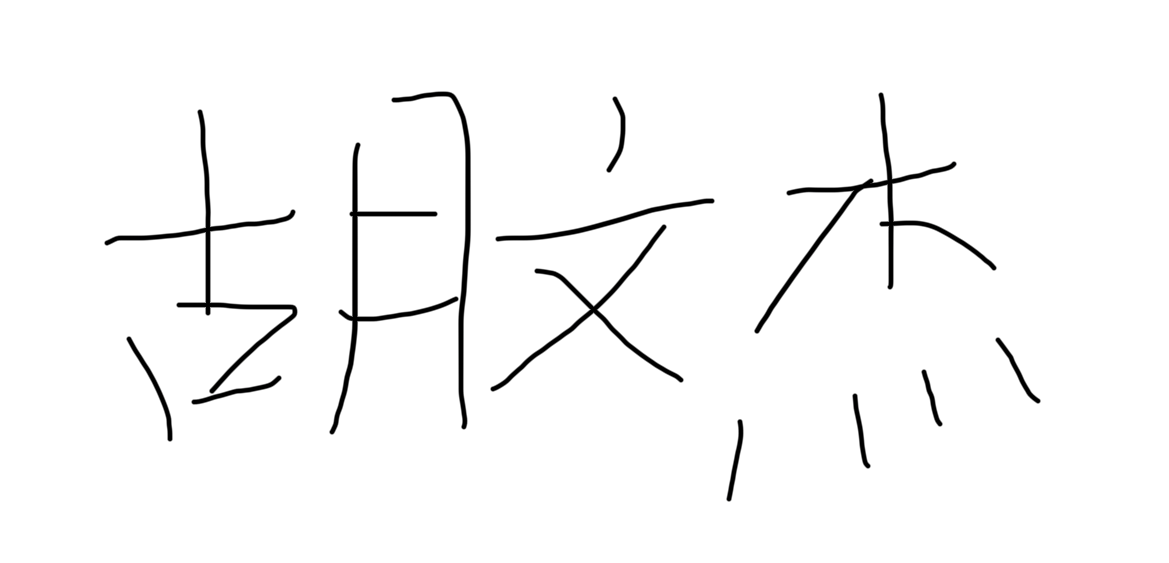
\includegraphics[height=1.0cm]{../my_signature.png}} \\
    日期：2026 年 5 月 8 日
  \end{tabular}
\end{flushright}

}

%TC:endignore

\end{document}
